\documentclass[12pt, a4paper]{article}

\usepackage{graphicx}
%\usepackage{subcaption}
\graphicspath{ {./images/} }
%Tarih Ekleme
\usepackage[ddmmyyyy]{datetime}
\renewcommand{\dateseparator}{.}
\renewcommand{\figurename}{Şekil}
\renewcommand{\refname}{Kaynakça}
\renewcommand{\abstractname}{Özet}

\usepackage{ragged2e}
\usepackage{blindtext}

% Başlık stili
\usepackage{titling}
\pretitle{\begin{center}\LARGE\bfseries}
	\posttitle{\end{center}}

%Hafta1

\title{Artırılmış Gerçeklik Ansiklopedisi Raporu Hafta 2 }
\author{Hasan Tekin}
\date{\today}
%\date{\DTMnow}
%\date{\DTMnow}


\begin{document}
	\maketitle
	
	\begin{abstract}
		\begin{justify}
		Bu projenin amacı, Vuforia ve Unity kullanarak bir artırılmış \newline gerçeklik ansiklopedisi oluşturmaktır.   Projenin amacı, kullanıcıların artırılmış gerçeklik aracılığıyla etkileşimli bilgiye ulaşmasını sağlamaktır. Çalışmada, Vuforia ve Unity kullanılarak 3D modeller, metinler ve görseller içeren bir ansiklopedi oluşturulmuştur. Ansiklopedideki içerik türleri ve kullanıcı etkileşim düzeyleri incelenmiştir. Görüntü tanıma ve nesne tanıma algoritmaları kullanılmıştır. Çalışma, kullanıcıların artırılmış gerçeklik aracılığıyla bilgiye daha etkileşimli ve etkili bir şekilde ulaşabileceğini göstermiştir.Bu çalışma, artırılmış gerçeklik \newline teknolojisinin eğitim ve bilgi sunumu alanlarında yenilikçi ve etkili bir araç olduğunu ortaya koymaktadır.
	\end{justify}
		\textbf{Anahtar Kelimeler:} Artırılmış Gerçeklik, Vuforia, Unity,Ansiklopedi, 3D Modeller, Görüntü Tanıma

	\end{abstract}
	
	\section{Giriş}
	Artırılmış gerçeklik (AR) teknolojisi, kullanıcılara gerçek dünya ile dijital bilgileri birleştirerek etkileşimli deneyimler sunar. Bu çalışmanın motivasyonu, AR teknolojisini kullanarak bilgi sunumunu daha etkileşimli ve etkili hale getirmektir. Artırılmış gerçeklik ansiklopedisi projemiz, Vuforia ve Unity platformlarını kullanarak geliştirilmiştir. Amacımız, kullanıcıların gerçek dünya nesneleri ile etkileşimde bulunarak bilgiye ulaşmasını sağlamak ve bu sayede öğrenme sürecini daha ilgi çekici hale getirmektir.
	\section{VERİ/DENEYSEL ÇALIŞMA DÜZENEĞİ VEYA LİTERATÜR ARAŞTIRMASI}
	Vuforia, artırılmış gerçeklik deneyimleri geliştirmek için geniş bir özellik yelpazesi sunar ve Unity ile entegre çalışarak güçlü AR uygulamaları oluşturmayı sağlar. Projede kullanılan veri, çeşitli 3D modeller, metinler ve görsellerden oluşmaktadır. Bu veriler, ansiklopedinin içeriğini oluşturmak için titizlikle seçilmiş ve işlenmiştir. Kullanıcıların gerçek dünya nesneleri ile etkileşimde bulunarak bilgiye ulaşmasını sağlayan AR ansiklopedisi, eğitim ve bilgi \newline sunumunda yenilikçi bir yaklaşım sunar.
	\section{Yöntem}
	Bu çalışmada, Vuforia ve Unity kullanılarak artırılmış gerçeklik ansiklopedisi geliştirilmiştir. Vuforia'nın görüntü tanıma ve nesne tanıma özellikleri kullanılarak, gerçek dünya nesnelerinin tanımlanması ve bu nesnelerle etkileşimli bilgi sunumu sağlanmıştır. Ansiklopedinin içeriği, 3D modeller, metinler ve görsellerden oluşmaktadır. Bu içerikler, kullanıcıların artırılmış gerçeklik deneyimlerini zenginleştirmek amacıyla seçilmiş ve entegre edilmiştir. Sistemin işleyişi, bir görsel veya kod akış şeması ile desteklenmiş ve kullanıcıların AR deneyimini daha etkili kılmak için optimize edilmiştir. Bu yöntemin seçilmesinin nedeni, Vuforia ve Unity'nin birlikte çalışarak güçlü ve etkileşimli AR deneyimleri sunma kapasitesidir.
	\subsection{Vuforia Nedir ?}
	
	Vuforia, artırılmış gerçeklik (AR) deneyimleri geliştirmek için kullanılan bir platformdur. Geliştiricilere, mobil cihazlar, tabletler ve akıllı gözlükler gibi cihazlarda çalışan interaktif AR uygulamaları oluşturma imkanı sağlar.
	
	Vuforia, birçok farklı endüstride kullanılabilecek geniş bir özellik yelpazesine sahiptir. Ürün tanıtımından eğitim ve eğlenceye kadar birçok farklı alan için kullanılabilir. Örneğin, Vuforia ile bir şirket ürününü interaktif bir şekilde sergileyebilir veya bir eğitim uygulamasında belirli nesnelerin tanımlanmasını sağlayabilirsiniz.
	
	Bu platform, görüntü tanıma, nesne tanıma, işaretleme ve bulut tabanlı hizmetler gibi çeşitli AR teknolojilerini destekler.Vuforia, Unity ve diğer popüler oyun motorlarıyla entegre olabilen bir geliştirme platformudur, bu da geliştiricilerin AR deneyimlerini oluşturmak için geniş bir araç yelpazesinden yararlanmalarını sağlar\cite{Vuforia}.
	\subsection{Unity Nedir ?}
	Unity, çok platformlu bir oyun motoru ve geliştirme ortamıdır. Unity Technologies tarafından geliştirilen bu araç, özellikle oyun geliştirme, simülasyonlar, mimari görselleştirmeler ve etkileşimli 3D içerik oluşturma gibi geniş bir yelpazede kullanım imkanı sunar.
	
	\subsection{Vuforia Nasıl Kullanılır ?}
	
	
	\newpage
	\begin{figure}[!ht]
		\caption{}
		\centering
		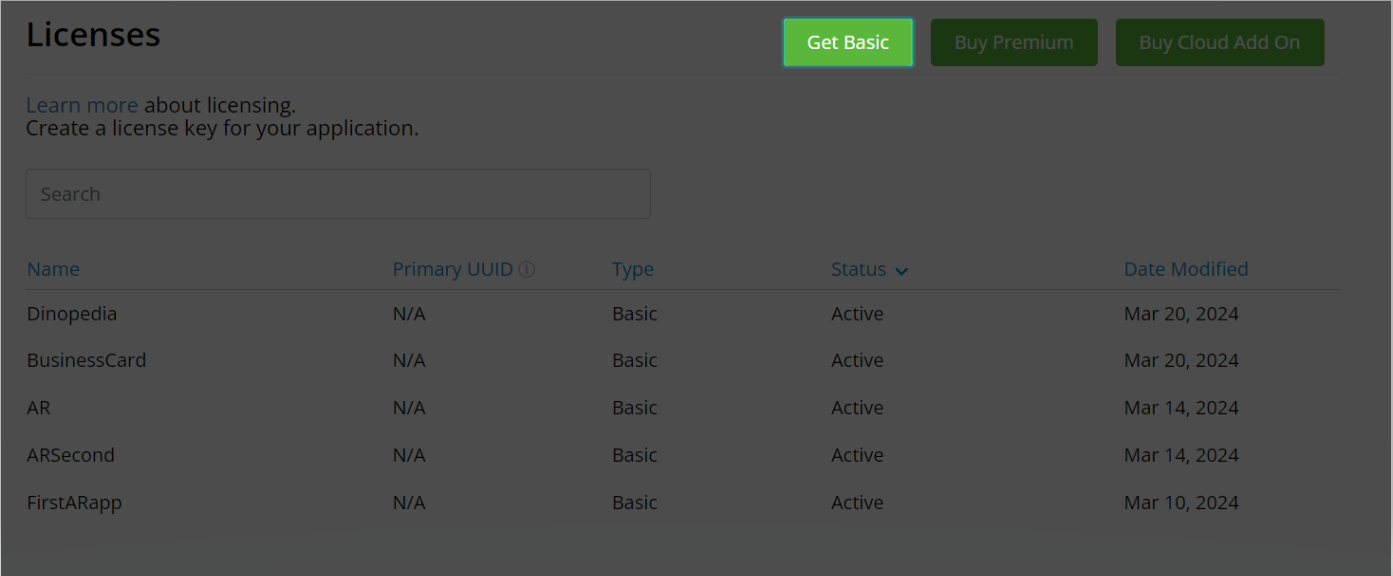
\includegraphics[angle=0, width=\textwidth]{Vuforia2.PNG}
		\label{gantt}
		Şekil \ref{gantt} de lisans sayfası gösterilmiştir\cite{Vuforia}.	
		
		
		
	\end{figure}
	
	\begin{figure}[!ht]
		\caption{}
		\centering
		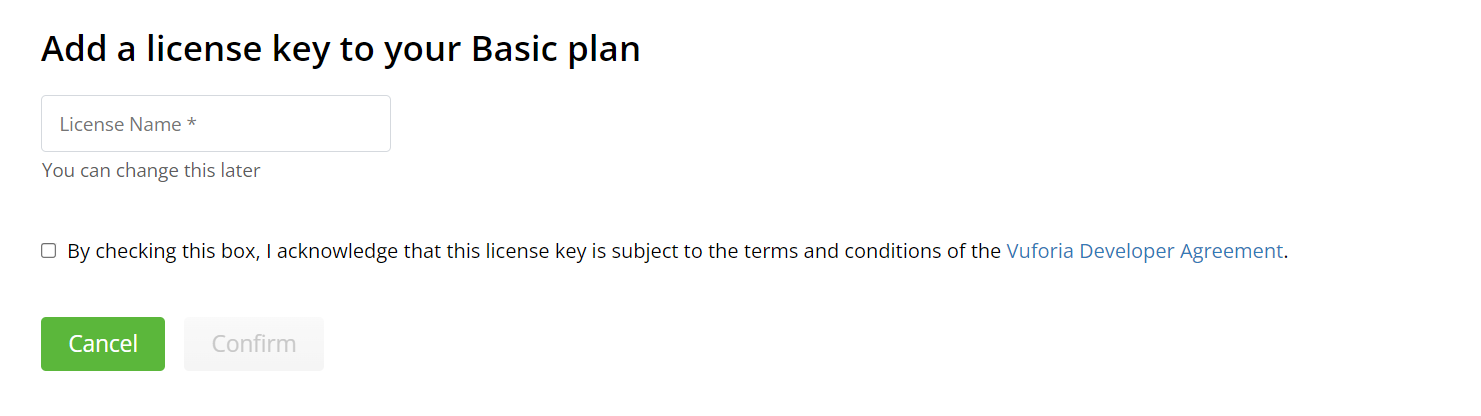
\includegraphics[angle=0, width=\textwidth]{Vuforia3.PNG}
		
		\label{gantt1}
		Şekil \ref{gantt1} de lisans sayfasında yeni bir lisans oluşturmanın ilk adımı gösterilmiştir\cite{Vuforia}.	
		
		
	\end{figure}
	\newpage
	\begin{figure}[!ht]
		\caption{}
		\centering
		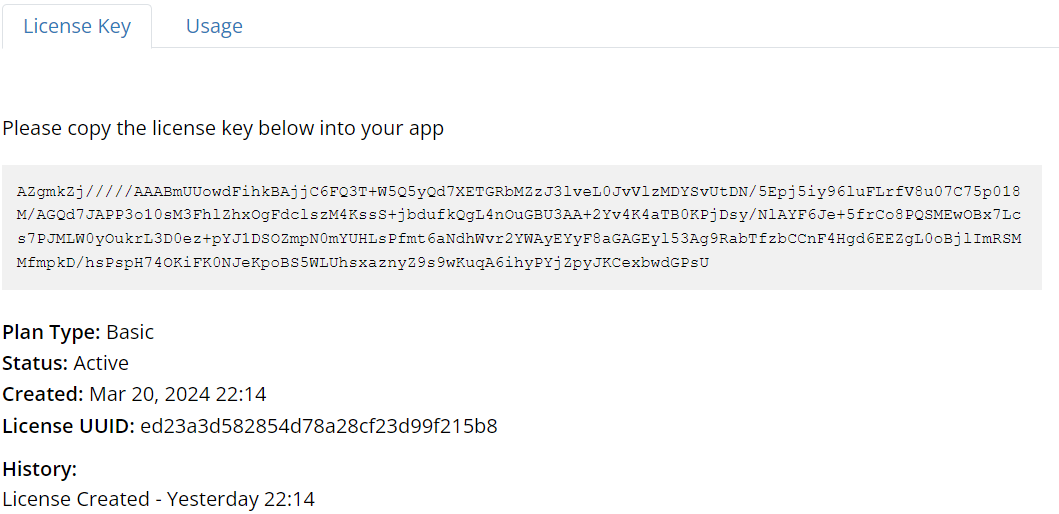
\includegraphics[angle=0, width=\textwidth]{Vuforia4.PNG}
		
		\label{gantt2}
		Şekil \ref{gantt2} de oluşturulan lisans gösterilmiştir\cite{Vuforia}.	
	\end{figure}
	
	\begin{figure}[!ht]
		\caption{}
		\centering
		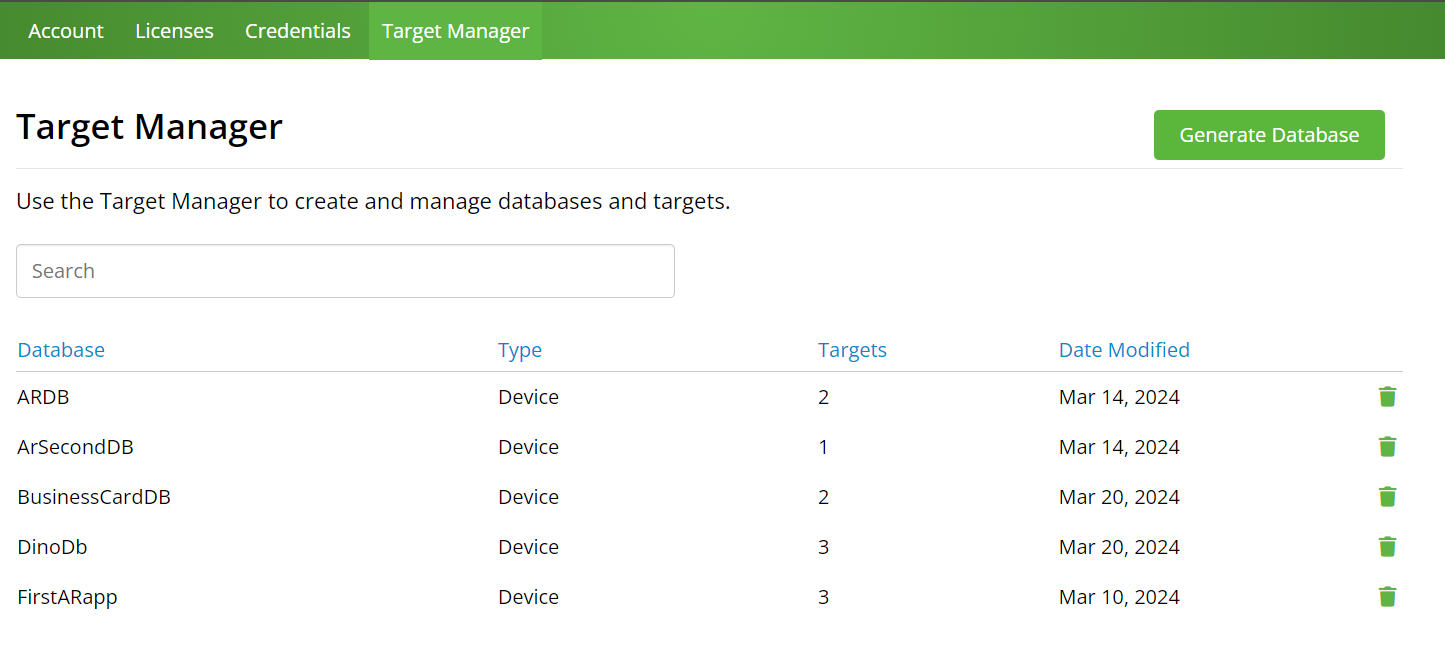
\includegraphics[angle=0, width=\textwidth]{Vuforia5.PNG}
		
		\label{gantt3}
		Şekil \ref{gantt3} de Target Manager için database oluşturma penceresi gösterilmiştir\cite{Vuforia}.	
	\end{figure}
	\newpage
	\begin{figure}[!ht]
		\caption{}
		\centering
		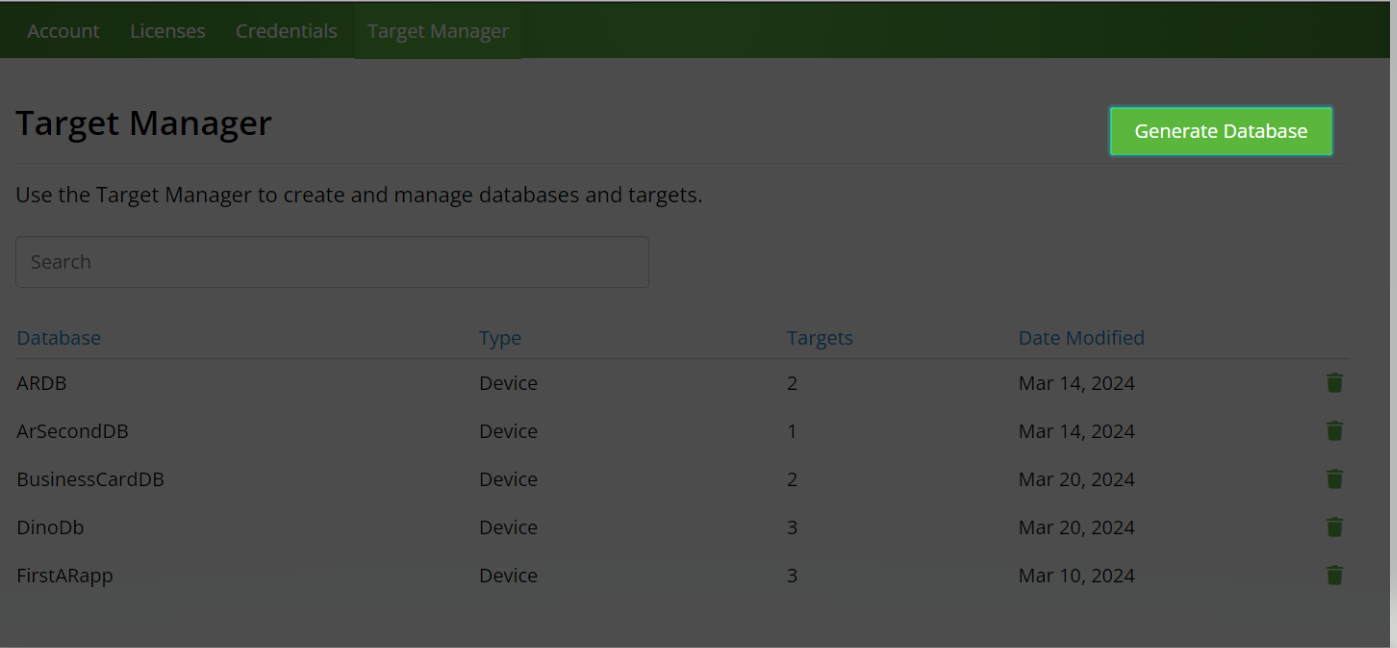
\includegraphics[angle=0, width=\textwidth]{Vuforia6.PNG}
		
		\label{gantt4}
		Şekil \ref{gantt4} de Target Manager için database oluşturmanın ilk adımı gösterilmiştir\cite{Vuforia}.	
	\end{figure}
	\begin{figure}[!ht]
		\caption{}
		\centering
		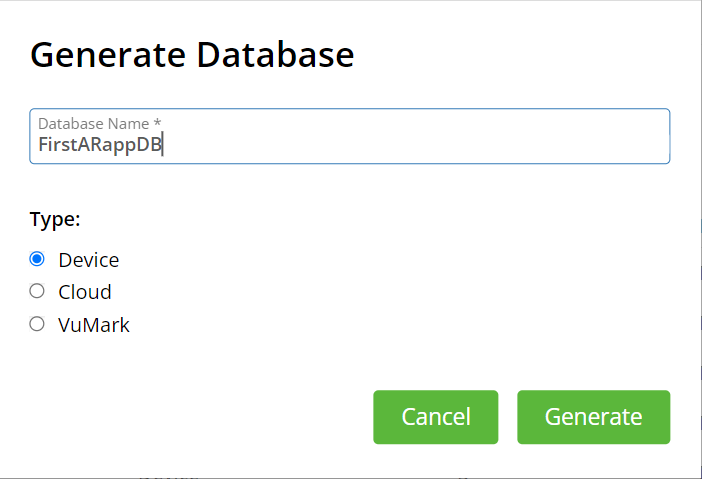
\includegraphics[angle=0, width=\textwidth]{Vuforia7.PNG}
		
		\label{gantt5}
		Şekil \ref{gantt5} de  database ismini verdiğimiz pencere gösterilmiştir\cite{Vuforia}.	
	\end{figure}
	\begin{figure}[!ht]
		\caption{}
		\centering
		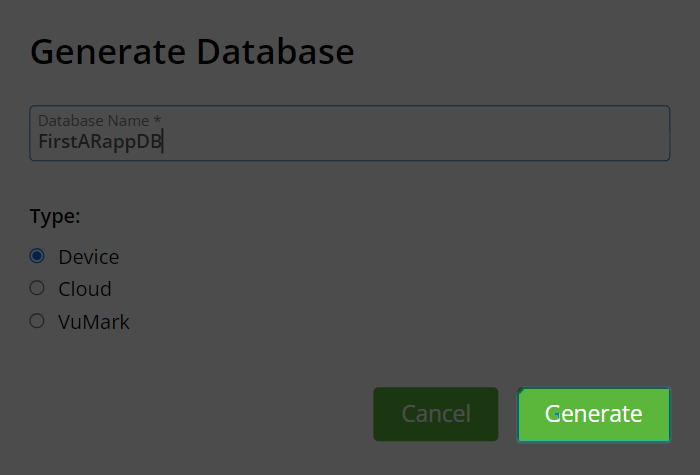
\includegraphics[angle=0, width=\textwidth]{Vuforia8.PNG}
		
		\label{gantt6}
		Şekil \ref{gantt6} de  database ismini verdikten sonra yapılacak işlem gösterilmiştir\cite{Vuforia}.	
	\end{figure}
	\newpage
	\begin{figure}[!ht]
		\caption{}
		\centering
		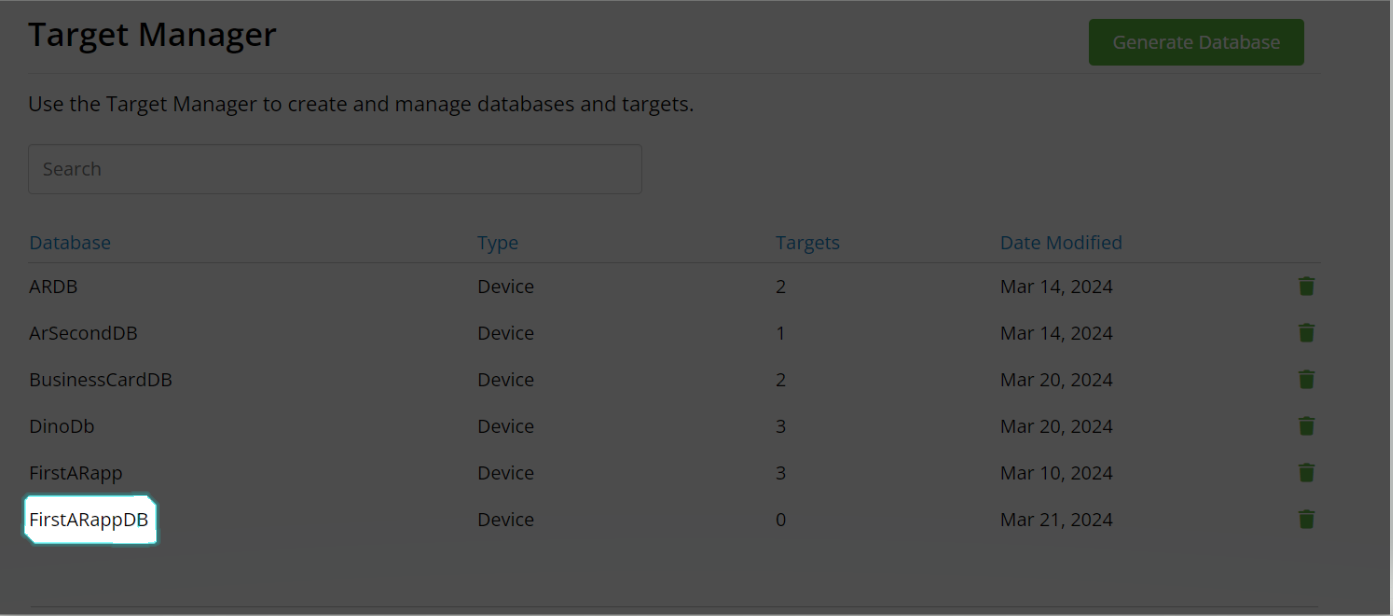
\includegraphics[angle=0, width=\textwidth]{Vuforia9.PNG}
		
		\label{gantt7}
		Şekil \ref{gantt7} de oluşturduğumuz databese gösterilmiştir\cite{Vuforia}.	
	\end{figure}
	\newpage
	\begin{figure}[!ht]
		\caption{}
		\centering
		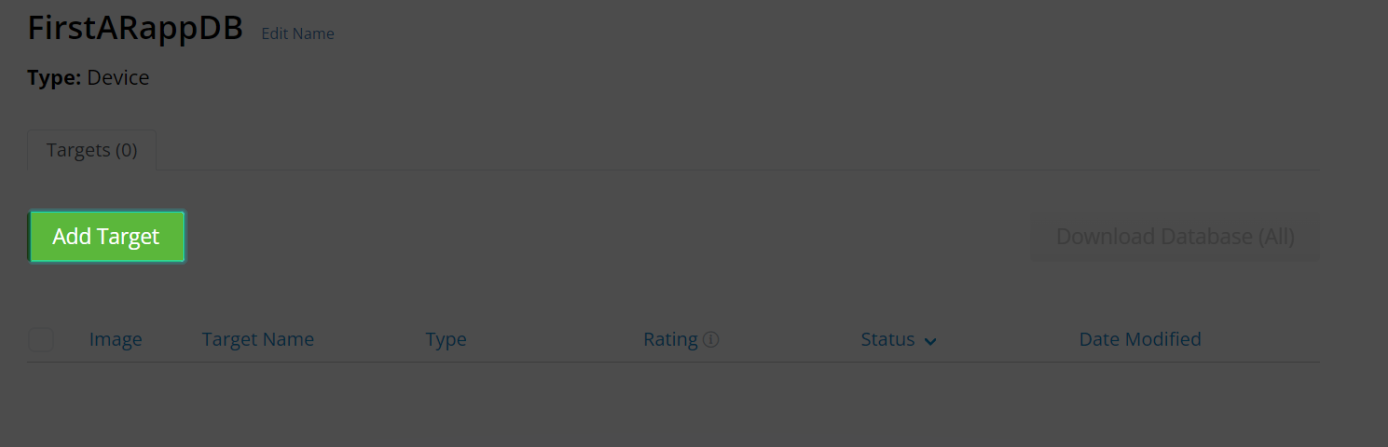
\includegraphics[angle=0, width=\textwidth]{Vuforia10.PNG}
		
		\label{gantt8}
		Şekil \ref{gantt8} de target eklemek istediğimizde kullanılacak kısım gösterilmiştir\cite{Vuforia}.	
	\end{figure}
	\newpage
	\begin{figure}[!ht]
		\caption{}
		\centering
		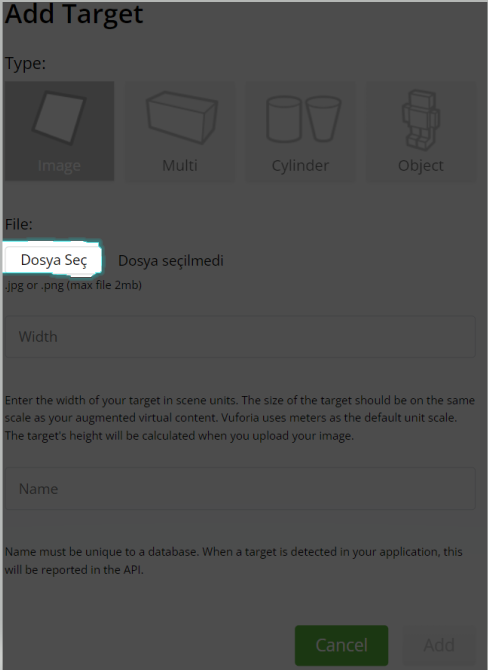
\includegraphics[angle=0, width=\textwidth]{Vuforia12.PNG}
		
		\label{gantt9}
		Şekil \ref{gantt9} de eklemek istediğimiz target seçme işlemi gösterilmiştir\cite{Vuforia}.	
	\end{figure}
	\begin{figure}[!ht]
		\caption{}
		\centering
		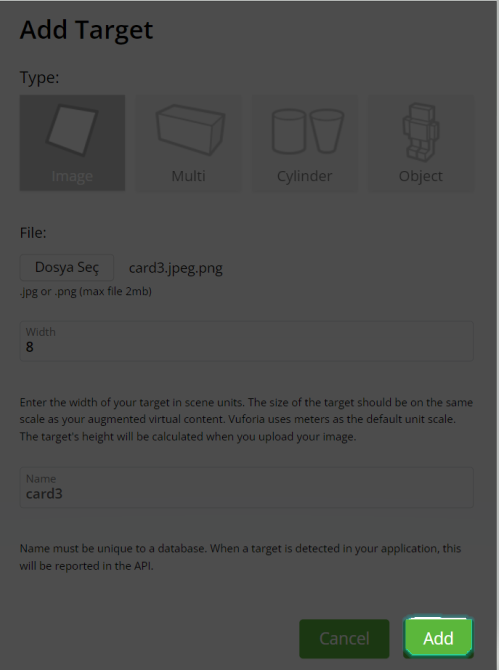
\includegraphics[angle=0, width=\textwidth]{Vuforia13.PNG}
		
		\label{gantt10}
		Şekil \ref{gantt10} de target eklemenin son adımı gösterilmiştir\cite{Vuforia}.
	\end{figure}
	\begin{figure}[!ht]
		\caption{}
		\centering
		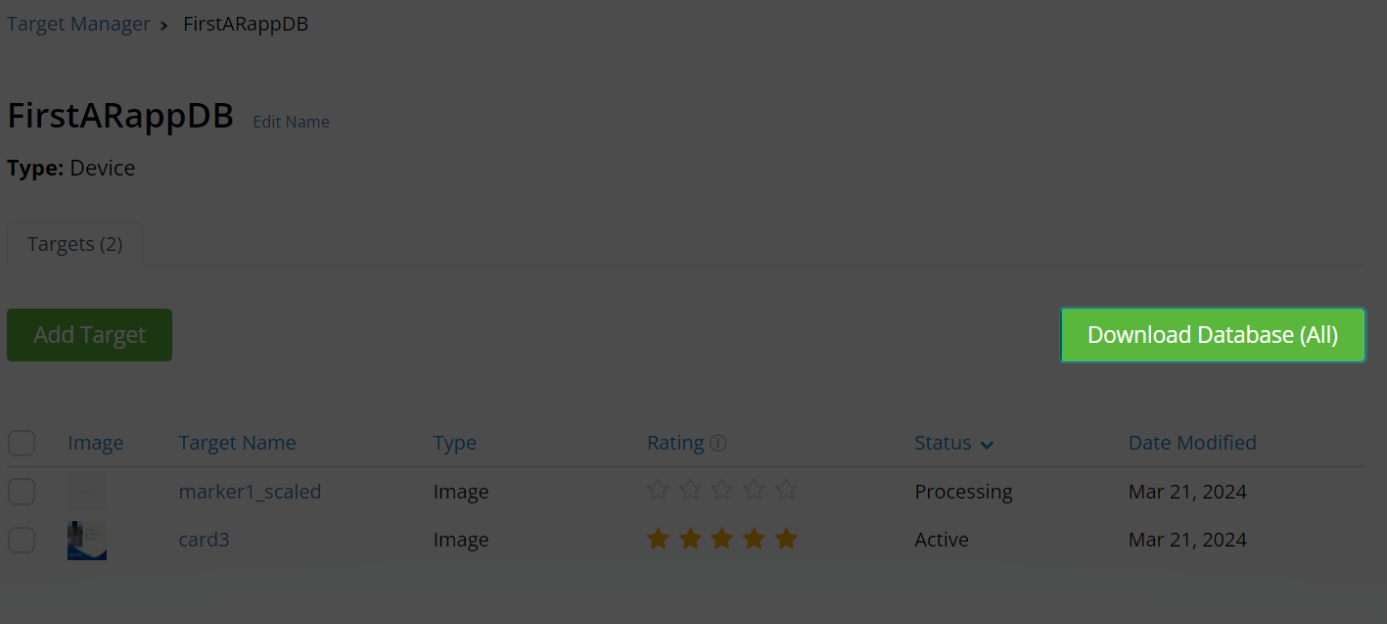
\includegraphics[angle=0, width=\textwidth]{Vuforia14.PNG}
		
		\label{gantt11}
		Şekil \ref{gantt11} de oluşturduğumuz target indirmek için ilk adım gösterilmiştir\cite{Vuforia}.
	\end{figure}
	\newpage
	\begin{figure}[!ht]
		\caption{}
		\centering
		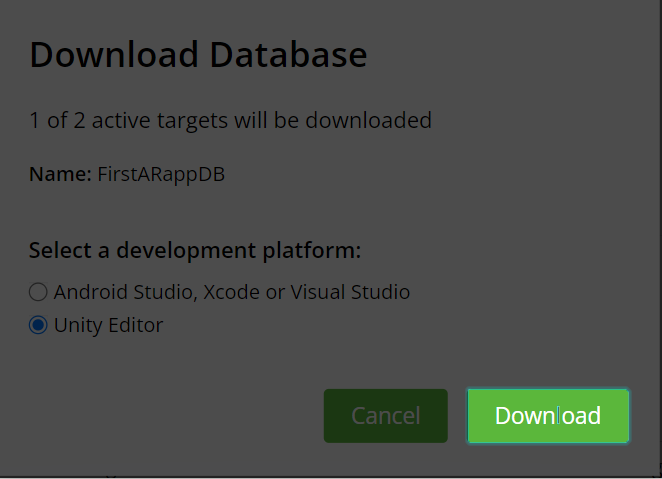
\includegraphics[angle=0, width=\textwidth]{Vuforia15.PNG}
		
		\label{gantt12}
		Şekil \ref{gantt12} de oluşturduğumuz target indirmek için son adım gösterilmiştir\cite{Vuforia}.
	\end{figure}
	\section{Sonuç}
	Bu çalışma, Vuforia ve Unity kullanarak artırılmış gerçeklik ansiklopedisi oluşturma sürecini ve sonuçlarını incelemektedir. AR ansiklopedisi, kullanıcıların gerçek dünya nesneleri ile etkileşimde bulunarak bilgiye ulaşmasını sağlayarak eğitim ve bilgi sunumunda yenilikçi bir yaklaşım sunmaktadır. Çalışmanın sonuçları, artırılmış gerçeklik teknolojisinin eğitim ve bilgi sunumu alanlarında yüksek etkileşim ve kullanıcı memnuniyeti sağladığını göstermektedir. Bu çalışma, AR teknolojisinin potansiyelini ortaya koymakta ve bu alandaki gelecekteki araştırmalara ışık tutmaktadır.
	\setcounter{section}{0}
	\newpage
		\title{Artırılmış Gerçeklikle Mobilya Görüntüleme Uygulaması Raporu Hafta 3}
	\author{}
	\date{}
	\maketitle
		\begin{abstract}
		\begin{justify}
		Bu çalışmanın amacı, kullanıcıların mobilya seçimlerini artırılmış gerçeklik (AR) aracılığıyla gerçek dünya mekanlarına yerleştirerek \newline görselleştirmelerini sağlayan bir uygulama geliştirmektir.Uygulama, mobilya alışverişi yapmadan önce kullanıcıların ürünlerin nasıl görüneceğini daha iyi anlamalarına yardımcı olur.Artırılmış Gerçeklik Ansiklopedisi uygulaması, kullanıcılara dünyada çok uzun zaman önce yaşamış  dinazorlar hakkında 3D modeller ve metinlerle bilgi sunmayı amaçlar.ARCore’un konum ve çevre algılama algoritmaları kullanılmıştır.Bu çalışma, AR teknolojisinin mobilya alışverişinde yenilikçi ve etkili bir araç olduğunu ortaya koymaktadır.  
		\end{justify}
		\textbf{Anahtar Kelimeler:}  Artırılmış Gerçeklik, ARCore, Mobilya \newline Görselleştirme, 3D Modeller, Gerçek Zamanlı Yerleştirme
		
	\end{abstract}
	\section{Giriş}
	Artırılmış gerçeklik (AR) teknolojisi, kullanıcıların dijital bilgileri gerçek dünya ile birleştirerek etkileşimli deneyimler sunmasını sağlar. Bu çalışmanın motivasyonu, kullanıcıların mobilya alışveriş deneyimini iyileştirmek ve doğru kararlar almalarını sağlamak için AR teknolojisini kullanmaktır. Furniture AR uygulaması, kullanıcıların seçtikleri mobilyaları sanal bir ortamda gerçek dünya mekanlarına yerleştirmelerine olanak tanır. Bu sayede, kullanıcılar mobilya alışverişi yapmadan önce ürünlerin nasıl görüneceğini daha iyi anlayabilirler.
	\section{Yöntem}
	Bu çalışmada, ARCore kullanılarak artırılmış gerçeklik mobilya uygulaması geliştirilmiştir. ARCore’un konum ve çevre algılama özellikleri kullanılarak, seçilen mobilyaların gerçek zamanlı olarak belirlenen mekanlara yerleştirilmesi sağlanmıştır. Uygulamanın içeriği, 3D mobilya modelleri ve görsellerden oluşmaktadır. Bu içerikler, kullanıcıların artırılmış gerçeklik deneyimlerini zenginleştirmek amacıyla seçilmiş ve entegre edilmiştir. Sistemin işleyişi, bir görsel veya kod akış şeması ile desteklenmiş ve kullanıcıların AR deneyimini daha etkili kılmak için optimize edilmiştir. Bu yöntemin seçilmesinin nedeni, ARCore’un mobil cihazlar üzerinde güçlü ve etkileşimli AR deneyimleri sunma kapasitesidir.
	\section{ BULGU ve TARTIŞMA}
	\begin{enumerate}
		\item 3D Mobilya Modelleri: Uygulama, kullanıcıların seçtikleri mobilyaları gerçek boyutta ve detaylı bir şekilde görmelerini sağlayan 3D modeller içerir.
		\item  Gerçek Zamanlı Yerleştirme: Kullanıcılar, mobil cihazlarını kullanarak seçtikleri mobilyaları gerçek zamanlı olarak belirledikleri mekanlara yerleştirebilirler\cite{drive}.
		
	\end{enumerate}
	\section{Sonuç}
	Bu çalışma, ARCore kullanarak artırılmış gerçeklik mobilya uygulaması \newline oluşturma sürecini ve sonuçlarını incelemektedir. AR mobilya uygulaması, kullanıcıların seçtikleri mobilyaları gerçek zamanlı olarak mekanlarına \newline yerleştirerek görselleştirmelerini sağlayarak alışveriş deneyiminde yenilikçi bir yaklaşım sunmaktadır.Bu çalışma, AR teknolojisinin potansiyelini ortaya koymakta ve bu alandaki gelecekteki araştırmalara ışık tutmaktadır.
	\newpage
	\begin{figure}[!htb]
		
		\begin{minipage}{0.48\textwidth}
			\centering
			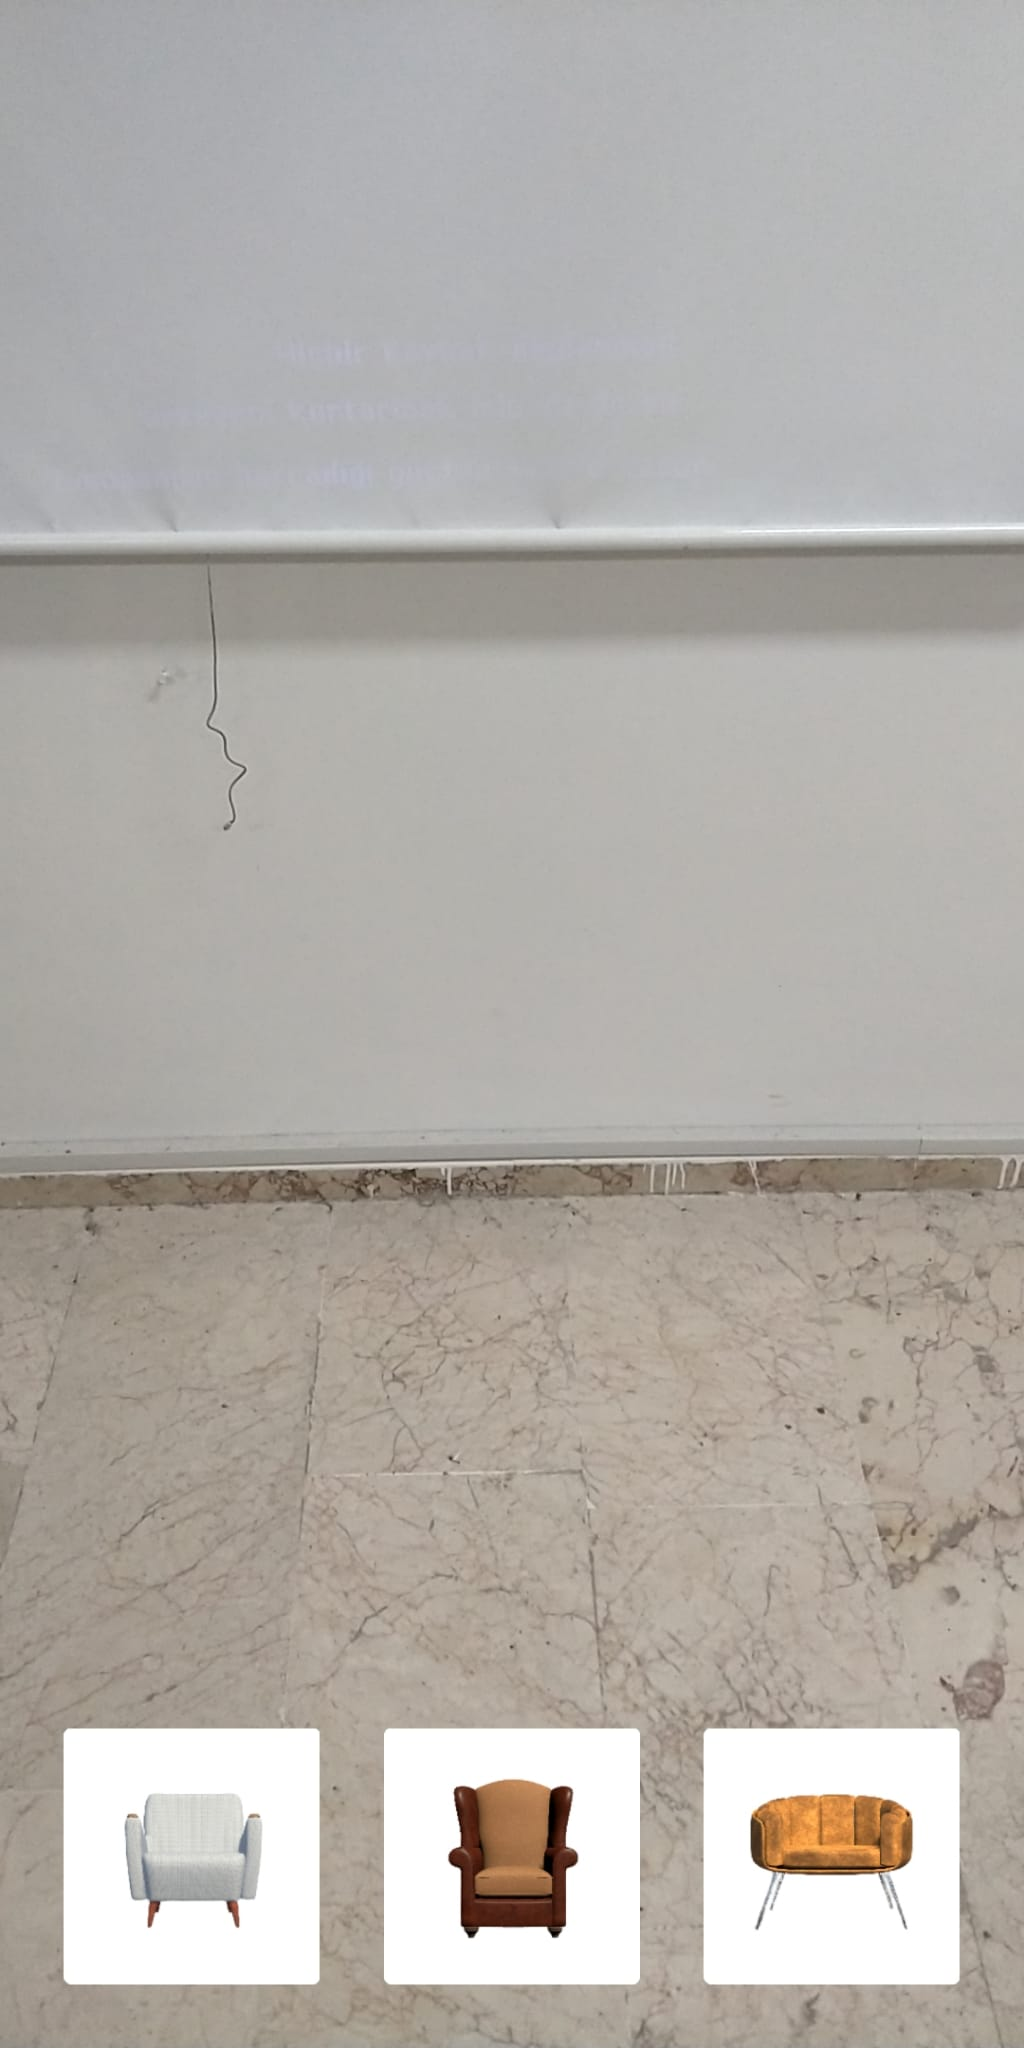
\includegraphics[width=.7\linewidth]{koltuk.jpeg}
			\caption{}\label{Fig:Data1}
		\end{minipage}\hfill
		\begin{minipage}{0.48\textwidth}
			\centering
			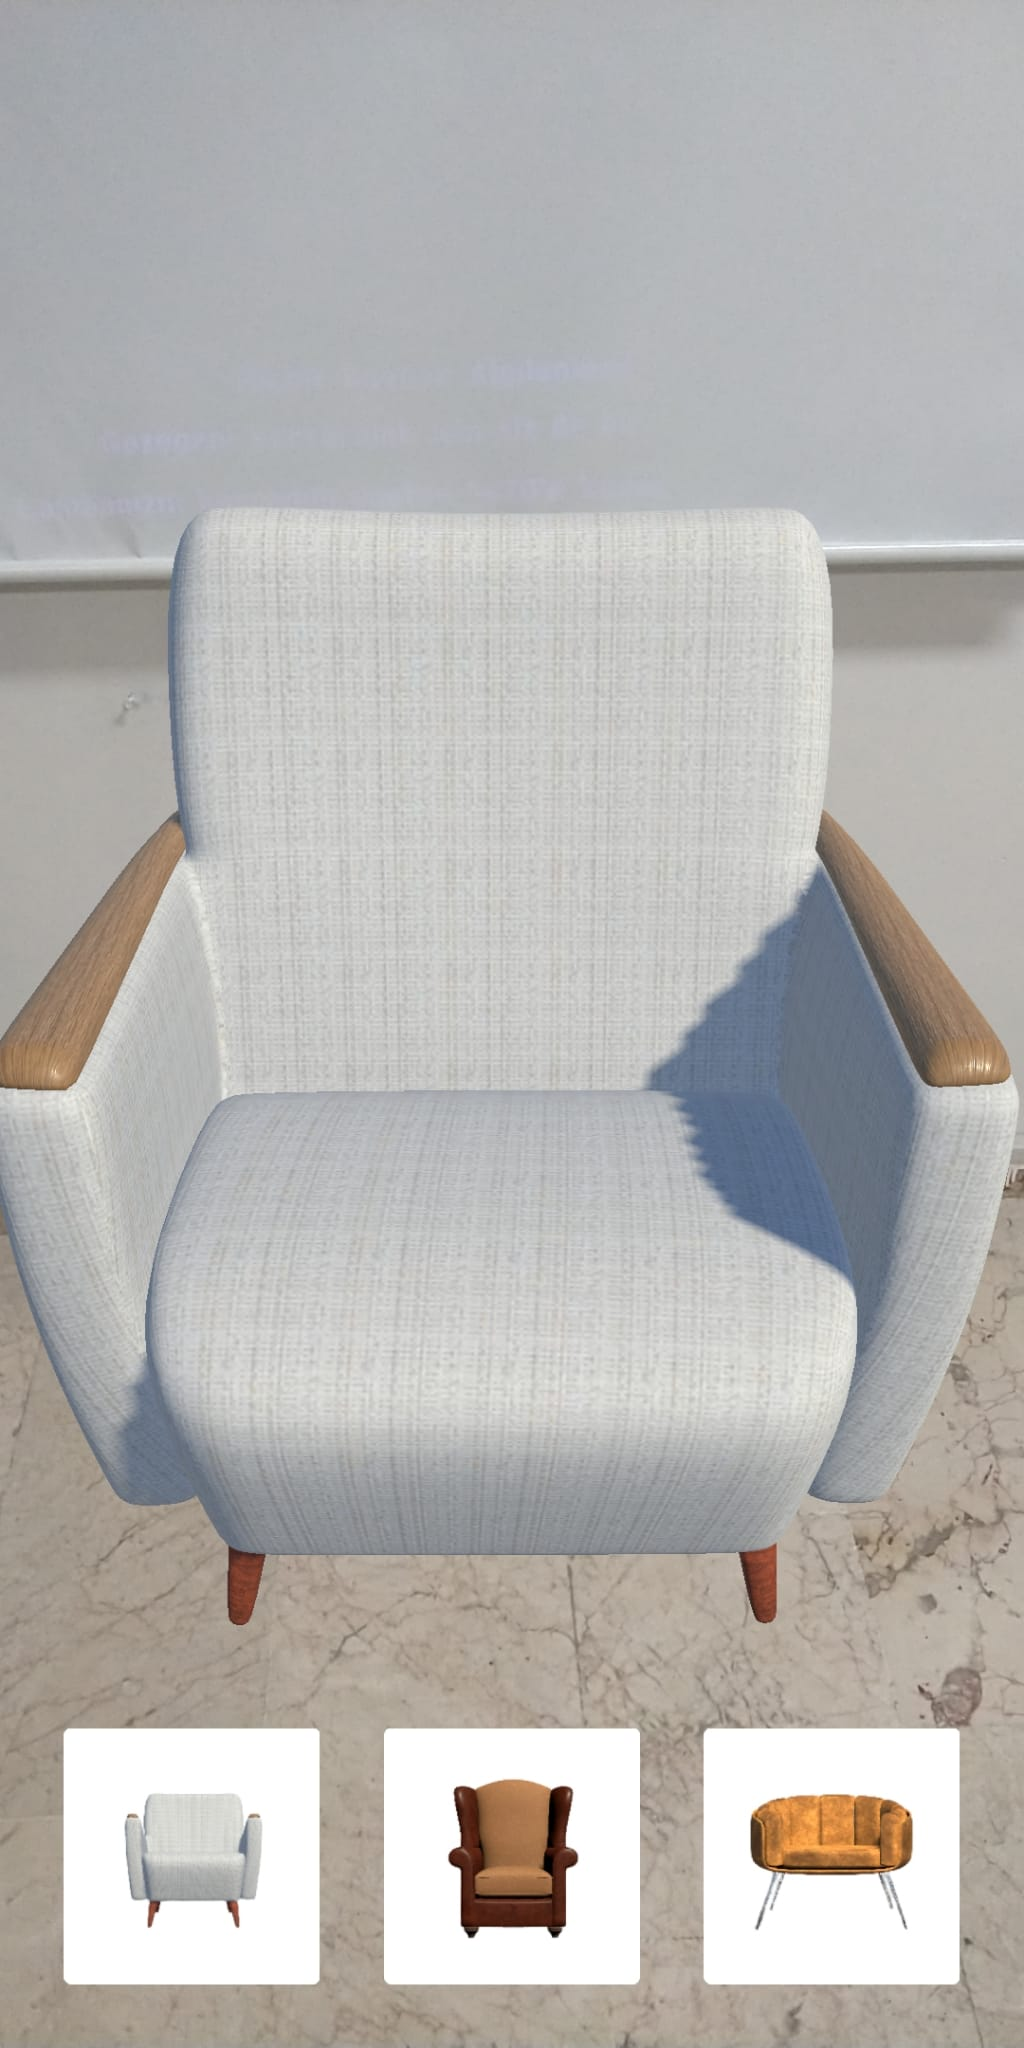
\includegraphics[width=.7\linewidth]{koltuk2.jpeg}
			\caption{}\label{Fig:Data2}
		\end{minipage}
	\end{figure}




	\newpage
		\title{Nuitrack Raporu Hafta 4}
	\author{Hasan Tekin}
	\date{\today}
	\maketitle
	
	\title{}
	\author{}
	\date{}
	\maketitle
		\setcounter{section}{0}
		\begin{abstract}
		\begin{justify}
		Bu çalışmanın amacı, 3DiVi Inc. tarafından geliştirilen Nuitrack yazılımını incelemektir.Nuitrack, Android, Windows ve Linux platformlarında Doğal Kullanıcı Arayüzü (NUI) yetenekleri sunan bir 3D izleme ve hareket tanıma yazılımıdır.Nuitrack, çeşitli endüstrilerdeki kullanıcılar için iskelet izleme ve hareket tanıma çözümleri sunarak interaktif uygulamaların geliştirilmesine olanak tanır.Nuitrack'in temel özellikleri ve kullanım alanları incelenmiştir.Nuitrack, 3D sensörlerle iletişim kuran algoritmalar kullanır..Nuitrack, AR/VR, tıbbi rehabilitasyon ve akıllı ev uygulamaları gibi birçok alanda etkili çözümler sunar.  
		\end{justify}
		\textbf{Anahtar Kelimeler:}Nuitrack, 3D İzleme, İskelet Takibi, Hareket Tanıma, Doğal Kullanıcı Arayüzü, 3D Sensörler
		
	\end{abstract}
	\section{Giriş}

	Nuitrack, 3DiVi Inc. tarafından geliştirilen ve 3D izleme, iskelet takibi ve hareket tanıma yetenekleri sunan bir yazılımdır. Bu çalışmanın motivasyonu, çeşitli platformlarda doğal kullanıcı arayüzü (NUI) yetenekleri sunan Nuitrack yazılımını incelemektir. Nuitrack, Android, Windows ve Linux işletim sistemlerinde çalışarak kullanıcıların iskelet izleme ve hareket tanıma gereksinimlerini karşılar. AR/VR uygulamaları, tıbbi rehabilitasyon ve akıllı ev sistemleri gibi birçok alanda kullanılabilecek geniş bir özellik yelpazesi sunar. Önceki çalışmalarda, Nuitrack'in çeşitli uygulama alanlarındaki etkinliği gösterilmiştir. Bu çalışmada, Nuitrack'in özellikleri, avantajları ve potansiyel uygulama alanları ele alınmaktadır \cite{3DiVi}.

	\newpage
	
	\section{Temel Özellikleri}
	\begin{enumerate}
		
		\item Tüm Vücut İskelet Takibi (19 Eklem)
		\begin{figure}[!ht]
			\caption{}
			\centering
			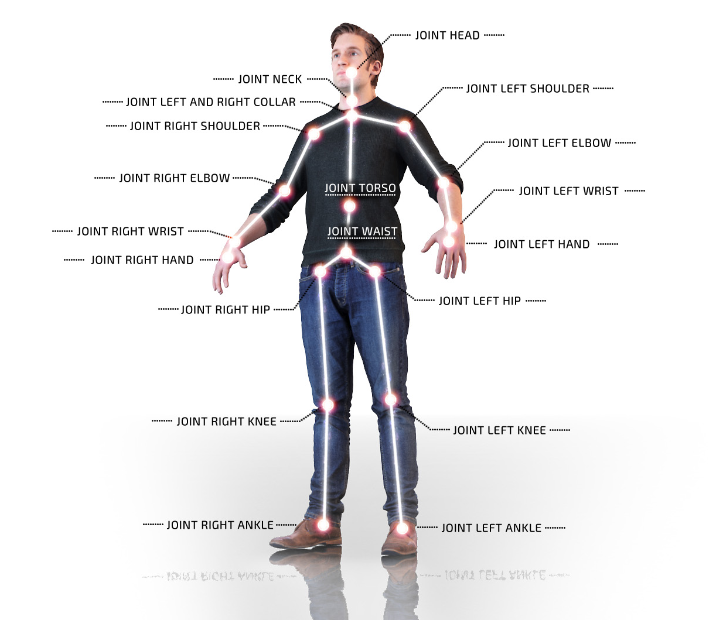
\includegraphics[width=0.8\textwidth]{Nuitrack.PNG}
			
			\label{dino1}
			Şekil \ref{dino1} de 19 eklem gösterilmiştir\cite{3DiVi}.	
		\end{figure}
		\newpage
		\item 3D Nokta Bulutu
		\begin{figure}[!ht]
			\caption{}
			\centering
			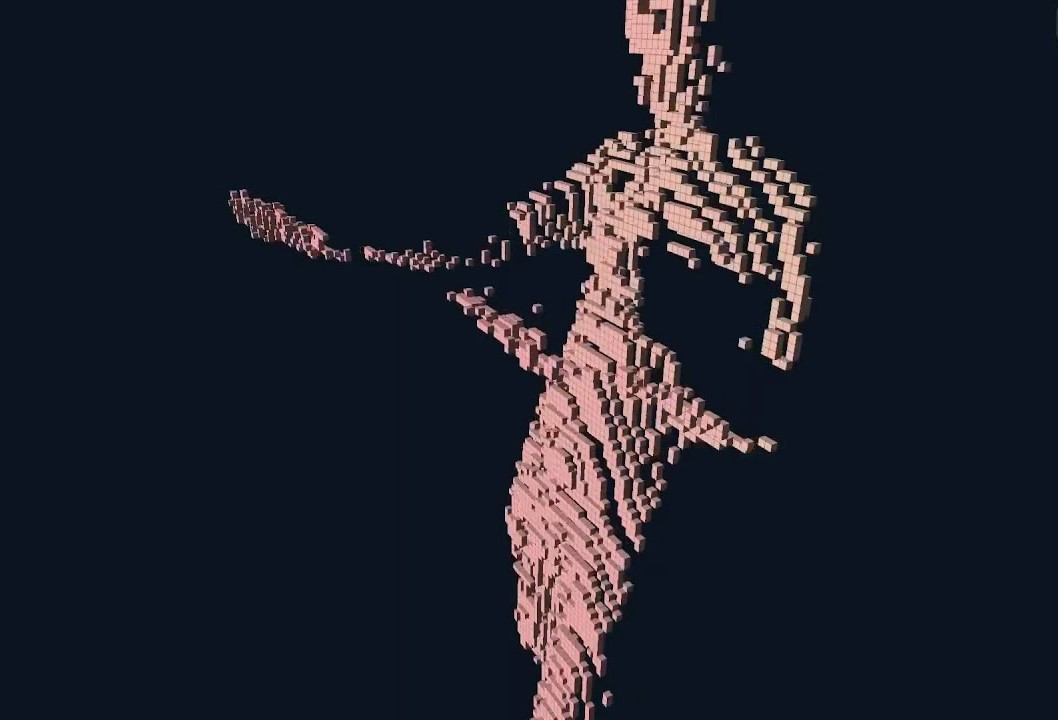
\includegraphics[width=0.8\textwidth]{Nuitrack1.jpg}
			
			\label{dino}
			Şekil \ref{dino1} de 3D nokta bulutu gösterilmiştir\cite{3dPointCloud}.	
		\end{figure}
		\item Kullanıcı Maskeleri
		\item Hareket Tanıma
		\item Android, Windows ve Linux için platformlar arası SDK
		\item 3D Sensör bağımsız Unity ve Unreal Engine Eklentileri
		\item OpenNI 1.5 uyumludur: OpenNI modülü, Kinect ve Asus Xtion için geliştirilen OpenNI tabanlı uygulamalarınızı Android dahil diğer platformlara taşımanıza olanak tanır\cite{3DiViBasic}.
		
	\end{enumerate}
	
	
	
	
	\section{Uygulama Alanları}
	\begin{enumerate}
		\item Windows/Linux/Android için Doğal Kullanıcı Arayüzü (NUI)
		\item Oyunlar ve Eğitim (Fitness, Dans Dersleri)
		\item Tıbbi Rehabilitasyon
		\item Akıllı Ev
		\item AR / VR için Tam Vücut Takibi
		\item Kitle Analitiği
		\item Robot Görüşü
		
		\cite{3DiViBasic}
		
	\end{enumerate}
	
	\section{Aldığım Hatalar}
	\begin{figure}[!ht]
		\caption{}
		\centering
		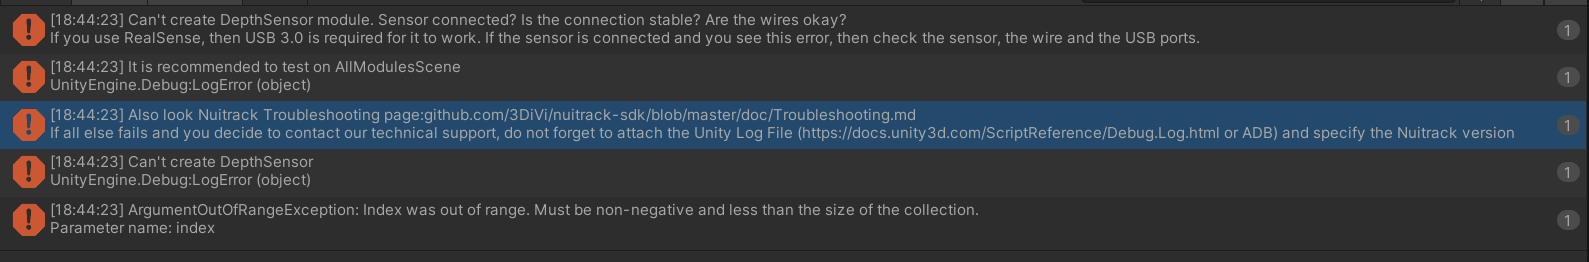
\includegraphics[width=0.8\textwidth]{unityHataPNG.PNG}
		
		\label{Hata}
		
	\end{figure}
	
	\newpage
	
	\title{Artırılmış Gerçeklik Raporu Hafta 5}
	\author{Hasan Tekin}
	\date{\today}
	\maketitle
	\setcounter{section}{0}
		\begin{abstract}
		\begin{justify}
			Artırılmış gerçeklik (AR) teknolojisi, yazılım endüstrisinde hızla büyüyen bir alan olup, çeşitli uygulamalarda kullanılmaktadır.AR uygulamaları geliştirmek, görüntü işleme, hareket izleme, uzamsal analiz ve makine öğrenimi gibi ileri düzeydeki algoritmaları gerektirir.Apple ve Android, AR uygulama geliştirme sürecini kolaylaştırmak için SDK'lar sunarken, Unity'nin AR Foundation kütüphanesi, bu süreci daha da basitleştirir.Bu çalışmanın amacı, AR Foundation'ın sağladığı avantajları ve kullanım alanlarını incelemektir.AR Foundation kullanılarak hem iOS hem de Android için tek bir kod tabanı ile AR uygulaması geliştirilebilir.AR Foundation, Apple ve Android SDK'larının entegrasyonunu sağlar.      
		\end{justify}
		\textbf{Anahtar Kelimeler:}Artırılmış Gerçeklik, AR Foundation, iOS, Android, SDK, Görüntü İşleme, Hareket İzleme
		
	\end{abstract}
	\section{Giriş}
	
	Artırılmış gerçeklik (AR), dijital bilgilerin gerçek dünya ile etkileşime girdiği ve kullanıcı deneyimlerini zenginleştirdiği bir teknolojidir. AR teknolojisi, makyaj simülasyonlarından kamera filtrelerine, sahne efektlerinden eğitim uygulamalarına kadar geniş bir kullanım yelpazesine sahiptir. Ancak, sıfırdan bir AR uygulaması geliştirmek, görüntü işleme, hareket izleme, uzamsal analiz ve makine öğrenimi gibi ileri düzeydeki algoritmalar hakkında bilgi gerektirir. Apple ve Android, bu süreci kolaylaştırmak için gerekli algoritmaları içeren SDK'lar geliştirmiştir. Ancak, her iki platform için ayrı ayrı uygulama geliştirmek, çabaları iki katına çıkarır. Bu sorunu çözmek için Unity, AR Foundation kütüphanesini geliştirmiştir. AR Foundation, tek bir kod tabanı ile hem iOS hem de Android için AR uygulamaları oluşturmayı mümkün kılar \cite{ARFoundation}.
	\section{AR FOUNDATION'IN TEMEL ÖZELLİKLERİ }
    AR Foundation, AR uygulama geliştirme sürecini basitleştiren ve hızlandıran birçok özellik sunar. Bu özellikler şunlardır:
    
    Platformlar Arası Destek: AR Foundation, tek bir kod tabanı ile hem iOS hem de Android platformları için AR uygulamaları geliştirme imkanı sağlar.
    Gelişmiş Algoritmalar: Görüntü işleme, hareket izleme, uzamsal analiz ve makine öğrenimi için gerekli algoritmaları içerir.
    Entegrasyon: Apple ve Android'in AR SDK'ları ile tam uyumlu çalışır.
    Kolay Kullanım: Geliştiricilerin, AR uygulamaları oluştururken karmaşık algoritmalarla uğraşmadan, daha hızlı ve verimli bir şekilde çalışmasını sağlar.
	\newpage
	\begin{figure}[!ht]
		\caption{}
		\centering
		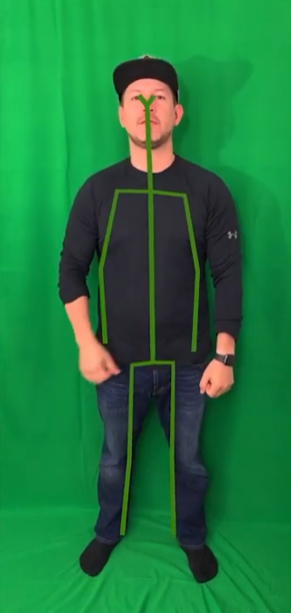
\includegraphics[height=0.8\textheight]{ARFoundation.PNG}
		
		\label{ARFoundation}
	\end{figure}
	Şekil \ref{ARFoundation} de gösterilen bu resim ARFoundation kullanılarak Gerçek Zamanlı Vücut İskeleti Oluşturmak için Vücut Takibi yapar\cite{Youtube}.
	
	
	
	
	
	\newpage
	\section{Uygulama Alanları}
		
		AR Foundation, birçok farklı alanda kullanılabilecek geniş bir uygulama yelpazesi sunar. Bu alanlar şunlardır:
		\begin{enumerate}
		\item Eğlence ve Medya: Kamera filtreleri, sahne efektleri ve oyunlar.
		\item Eğitim: Eğitim uygulamaları ve simülasyonlar.
		\item Perakende: Ürün görselleştirme ve sanal deneme odaları.
		\item Sağlık: Tıbbi simülasyonlar ve rehabilitasyon uygulamaları.
		\item Sanat ve Kültür: Müzelerde interaktif sergiler ve kültürel mirasın dijitalleştirilmesi.
	\end{enumerate}

    \section{SONUÇ}
    Bu çalışma, AR Foundation'ın artırılmış gerçeklik uygulama geliştirme \newline sürecini nasıl basitleştirdiğini ve platformlar arası uyumluluğu nasıl sağladığını incelemektedir. AR Foundation, geliştiricilerin tek bir kod tabanı ile hem iOS hem de Android için AR uygulamaları geliştirmesini mümkün kılarak, geliştirme sürecini önemli ölçüde kolaylaştırır. Çalışmanın sonuçları, AR Foundation'ın, AR uygulamalarının daha geniş bir kullanıcı kitlesine ulaşmasını sağladığını göstermektedir. Bu çalışma, AR Foundation'ın sağladığı avantajları ve potansiyel kullanım alanlarını ortaya koyarak, AR teknolojisinin gelecekteki gelişiminde önemli bir rol oynayacağını göstermektedir.
	
	\title{}
	\author{}
	\date{}
	\maketitle
	% Section değerini sıfırlıyor alt başlık değerini
	\setcounter{section}{0}
		\begin{abstract}
		\begin{justify}
		   MediaPipe, Google tarafından geliştirilen ve görüntü ile video işleme amacıyla kullanılan açık kaynaklı bir kütüphanedir.Bu kütüphane, işaret işleme, nesne algılama, yüz tanıma, el izleme ve vücut izleme gibi çeşitli görevlerde kullanılır.MediaPipe, gerçek zamanlı hareket takibi ve analizini kolaylaştırarak, geliştiricilere kapsamlı ve esnek çözümler sunar.Bu çalışmanın amacı, Unity ve MediaPipe kullanarak basit bir hareket takibi sistemi geliştirmektir.Kameradan gelen görüntüler işlenmiş ve kişinin vücudundaki eklemler tanımlanarak hareketler gerçek zamanlı olarak takip edilmiştir.İzlenen kişinin hareketlerinin doğruluğu ve takip performansı değerlendirilmiştir.MediaPipe'in vücut izleme algoritmaları kullanılmıştır.Çalışma, MediaPipe kullanılarak geliştirilen sistemin, gerçek zamanlı hareket takibinde yüksek doğruluk ve performans sunduğunu göstermiştir.MediaPipe, vücut izleme ve hareket takibi için etkili bir çözümdür. Diğer hareket takibi sistemleri ile karşılaştırıldığında, MediaPipe'in esnekliği ve doğruluğu öne çıkmaktadır.Bu çalışma, MediaPipe kullanarak geliştirilen basit bir hareket takibi sisteminin etkinliğini ve uygulama potansiyelini ortaya koymaktadır.
		\end{justify}
		\textbf{Anahtar Kelimeler:}MediaPipe, Hareket Takibi, Vücut İzleme, Unity, Görüntü İşleme, Video İşleme
		
	\end{abstract}
	\section{Giriş}
	MediaPipe, Google tarafından geliştirilen ve açık kaynaklı olarak sunulan bir kütüphanedir. Görüntü ve video işleme alanında geniş bir kullanım yelpazesi sunar. MediaPipe, işaret işleme, nesne algılama, yüz tanıma, el izleme ve vücut izleme gibi çeşitli işlemler için kullanılabilir. Bu çalışmanın motivasyonu, MediaPipe'in sağladığı gelişmiş görüntü işleme yeteneklerini kullanarak hareket takibi sistemleri geliştirmektir. MediaPipe, geliştiricilere, karmaşık görüntü işleme görevlerini basit ve verimli bir şekilde gerçekleştirme olanağı tanır. Bu çalışmada, MediaPipe'in özellikleri ve kullanım alanları incelenerek, Unity ile entegrasyon sağlanmış ve basit bir hareket takibi sistemi geliştirilmiştir.
	
	\begin{figure}[!ht]
		\caption{}
		\centering
		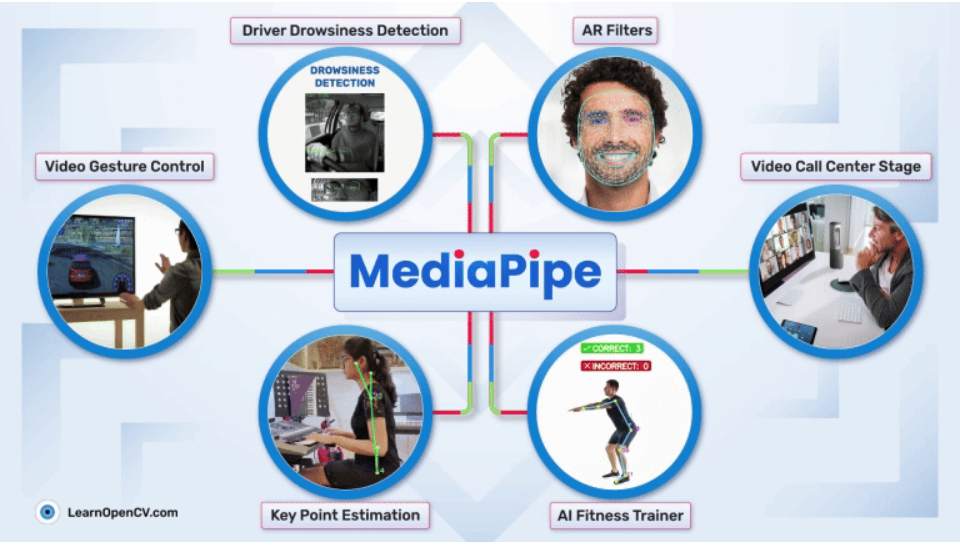
\includegraphics[width=0.8\textwidth]{mediaPipe.PNG}
		
		\label{mediaPipe}
	\end{figure}
	Şekil \ref{mediaPipe} de gösterilen bu görsel mediaPipe'ın kullanım alanlarını göstermektedir\cite{MediaPipe}.
	\newpage
	\section{MediaPipe Hareket Takibi Örneği}
	\begin{enumerate}
		\item Bu örneğin temel amacı, Unity ve MediaPipe kullanarak basit seviyede bir hareket takibi sistemi geliştirmektir. Bu örnekteki amaç bir kişinin hareketlerini gerçek zamanlı olarak izlemeyi hedeflemektedir. MediaPipe kullanılarak kameradan gelen görüntü işlenecek ve izlenen kişinin vücudundaki eklemler tanımlanarak hareketleri takip edilecektir.
		
	\end{enumerate}
	
	\subsection{Kullanılan Teknolojiler}
		\begin{enumerate}
      \item 	MediaPipe: MediaPipe, görüntü ve video işleme için kullanılan güçlü bir kütüphanedir. Bu kütüphane, gerçek zamanlı vücut izleme ve hareket takibi için gerekli algoritmaları içerir.
	\item Unity: Unity, 3D ve 2D oyunlar ile interaktif içerik geliştirmek için kullanılan popüler bir oyun motorudur. MediaPipe ile entegrasyonu, gerçek zamanlı hareket takibi uygulamaları geliştirmeyi kolaylaştırır
	\end{enumerate}
	\subsection{Hareket Takibi Sisteminin Geliştirilmesi}
	Bu örnekte, MediaPipe'in vücut izleme algoritmaları kullanılarak, bir kişinin vücudundaki eklemler tanımlanmış ve bu eklemlerin hareketleri gerçek zamanlı olarak takip edilmiştir. Sistemin geliştirilme süreci şu adımlardan oluşmaktadır:
	\begin{enumerate}
	\item	Görüntü Alımı: Kameradan gelen görüntüler alınır ve MediaPipe tarafından işlenir.
	\item	Vücut İskeletinin Tanımlanması: MediaPipe, kameradan gelen görüntülerdeki kişiyi tanımlar ve vücudundaki eklemleri belirler.
	\item	Hareket Takibi: Tanımlanan eklemler üzerinden kişinin hareketleri gerçek zamanlı olarak izlenir ve takip edilir.
	\end{enumerate}
	\begin{figure}[!ht]
		\caption{}
		\centering
		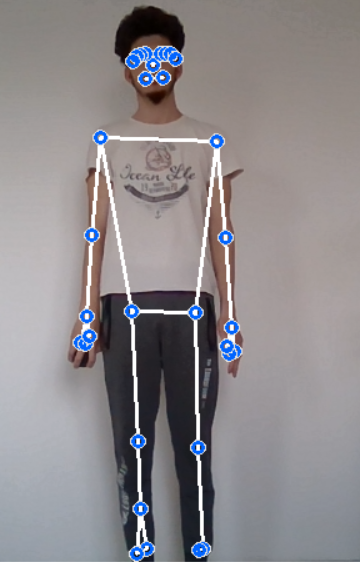
\includegraphics[height=0.8\textheight]{Ben2.png}
		
	
	\label{Ben}
	\end{figure}
	\newpage
	Şekil \ref{Ben} de gösterilen bu görselde eklemler gösterilmektedir.
	\begin{figure}[!ht]
		\caption{}
		\centering
		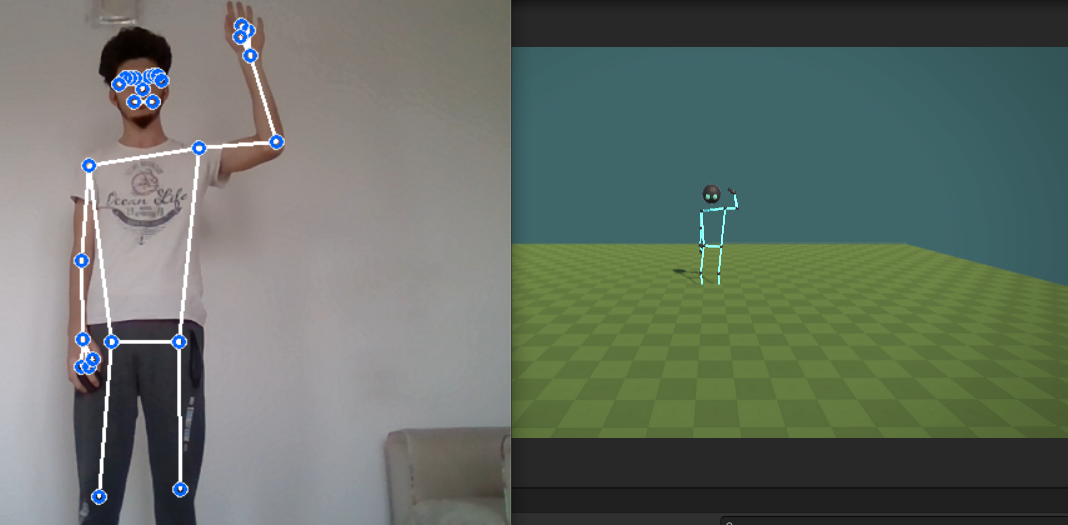
\includegraphics[width=0.8\textwidth]{Klon.PNG}
		
		\label{Klon}
	\end{figure}
	\newpage
	Şekil \ref{Klon} de gösterilen bu görselde gerçek zamanlı hareket gösterilmektedir.
	\newpage
\section{Sonuç}
Bu çalışma, MediaPipe kullanarak geliştirilen basit bir hareket takibi sisteminin etkinliğini ve uygulama potansiyelini ortaya koymaktadır. MediaPipe, gerçek zamanlı hareket takibi ve vücut izleme için etkili bir çözüm sunarak, geliştiricilere geniş bir uygulama yelpazesi sunmaktadır. Unity ile entegrasyonu, hareket takibi uygulamalarını daha hızlı ve verimli bir şekilde geliştirmeyi mümkün kılmaktadır. Bu çalışma, MediaPipe'in sağladığı avantajları ve potansiyel kullanım alanlarını vurgulayarak, gelecekteki projeler için temel bir kaynak oluşturmaktadır.
\newpage
\title{Tişört Seçme Uygulaması Raporu
	Hafta 6}
\author{}
\date{}
\maketitle
\setcounter{section}{0}
\begin{abstract}
	\begin{justify}
		Tişört Seçme Uygulaması, kullanıcıların farklı tişörtleri sanal olarak denemesine olanak tanıyan bir bilgisayarda görü tabanlı sistemdir.Bu sistem, kullanıcıların fiziksel olarak tişört denemeden nasıl görüneceğini görselleştirmelerine yardımcı olur.Uygulama, vücut pozunu ve eklem noktalarını algılayarak, kullanıcı deneyimini iyileştirir.Vücut pozunun doğruluğu ve tişört yerleştirme başarısı değerlendirilmiştir.   
		
	\end{justify}
	\textbf{Anahtar Kelimeler:}  Tişört Seçme Uygulaması, OpenCV, CVZone, Sanal Deneme, Bilgisayarla Görü, MediaPipe
\end{abstract}
\section{Giriş}
Tişört Seçme Uygulaması, kullanıcıların farklı tişörtleri sanal olarak denemelerine olanak tanıyan bir bilgisayar görüsü tabanlı sistemdir. Bu uygulama, kullanıcıların önceden kaydedilmiş bir video kullanarak farklı tişörtleri sanal olarak denemelerini sağlar. Vücut pozunu ve eklem noktalarını algılayarak, farklı tişört görüntülerini kullanıcının bedenine ekler. Bu sayede kullanıcılar, fiziksel olarak tişört denemeden nasıl görüneceklerini görselleştirebilirler. Bu çalışmanın motivasyonu, kullanıcı deneyimini iyileştirerek, sanal deneme süreçlerini daha etkili hale getirmektir \cite{Tisort}.
\section{OpenCV ve CVZone}
\subsection{OpenCV Nedir?}
OpenCV (Open Source Computer Vision Library), gerçek zamanlı bilgisayar görüsü uygulamalarında kullanılan açık kaynaklı bir kütüphanedir. İlk olarak Intel tarafından geliştirilmiş olup, daha sonra Willow Garage ve Itseez tarafından sürdürülmüştür. OpenCV, çoklu platform desteği sunar ve BSD lisansı altında açık kaynaklı bir yazılımdır. Bu kütüphane, görüntü işleme ve analizinde geniş bir işlevsellik sunar.
 \begin{figure}[!ht]
	\caption{}
	\centering
	
\includegraphics[angle=0, width=\textwidth]{OpenCv.jpg}
	\label{OpenCv}
	Şekil \ref{OpenCv} de OpenCv logosu gösterilmiştir\cite{OpenCvResim}.	
	
	
	
\end{figure}
\newpage
\subsection{CVZone Nedir?}
CVZone, görüntü işleme ve yapay zeka işlevlerini çalıştırmayı kolaylaştıran bir bilgisayarla görü paketidir. Temelde OpenCV ve MediaPipe kütüphanelerini kullanır. CVZone, geliştiricilere, bilgisayarla görüsü tabanlı projelerde hızlı ve etkili çözümler sunar.
 \begin{figure}[!ht]
	\caption{}
	\centering
	
\includegraphics[angle=0, width=\textwidth]{CVZone.png}
	\label{CVZone}
	Şekil \ref{CVZone} de CVZone logosu gösterilmiştir\cite{CVZoneResim}.	
	
	
	
\end{figure}
\section{CVZone Kullanarak Tişört Seçme Uygulaması}
\subsection{Kullanılan Teknolojiler}
\begin{enumerate}
	\item OpenCV: Gerçek zamanlı görüntü işleme için kullanılan temel kütüphane.
	\item MediaPipe: Vücut pozunu ve eklem noktalarını algılamak için kullanılan kütüphane.
	\item CVZone: OpenCV ve MediaPipe entegrasyonunu sağlayarak, uygulamanın geliştirilmesini kolaylaştırır. 
\end{enumerate}
\subsection{Uygulamanın Geliştirilmesi}
Bu uygulamanın temel amacı, kullanıcıların farklı tişörtleri sanal olarak denemelerine olanak tanımaktır. Aşağıda, uygulamanın geliştirilme süreci ve kullanılan yöntemler detaylandırılmaktadır:
\begin{enumerate}
	\item Görüntü Alımı: Kullanıcının önceden kaydedilmiş video görüntüleri alınır ve işlenir.
	\item Vücut Pozunun Algılanması: MediaPipe kullanılarak, kullanıcının vücut pozisyonu ve eklem noktaları algılanır.
	
	\item Tişört Yerleştirme: Algılanan eklem noktaları kullanılarak, seçilen tişört görüntüsü kullanıcının bedenine yerleştirilir.
	\item 	Gerçek Zamanlı Görselleştirme: Kullanıcı, sanal olarak denediği tişörtleri gerçek zamanlı olarak görebilir.
	
	 
\end{enumerate}
\section{Sonuç}
 Bu çalışma, OpenCV ve CVZone kullanarak sanal tişört denemelerinde etkin bir çözüm sunmaktadır. Geliştirilen sistem, kullanıcıların fiziksel olarak tişört denemeden farklı tişörtlerin nasıl görüneceğini görselleştirmelerine olanak tanır. OpenCV ve MediaPipe'in entegrasyonu, hareket takibi ve vücut pozisyonu algılamada yüksek doğruluk sağlar.
 	\section{Beklenen Çıktı}
 
 \newpage
 \begin{figure}[!ht]
 	\caption{}
 	\centering
 	\includegraphics[angle=0, width=\textwidth]{gomlek1.PNG}
 	\label{gomlek1}
 	Şekil \ref{gomlek1} de ilk tişört gösterilmiştir\cite{TisortPackage}.	
 	
 	
 	
 \end{figure}
 
 \begin{figure}[!ht]
 	\caption{}
 	\centering
 	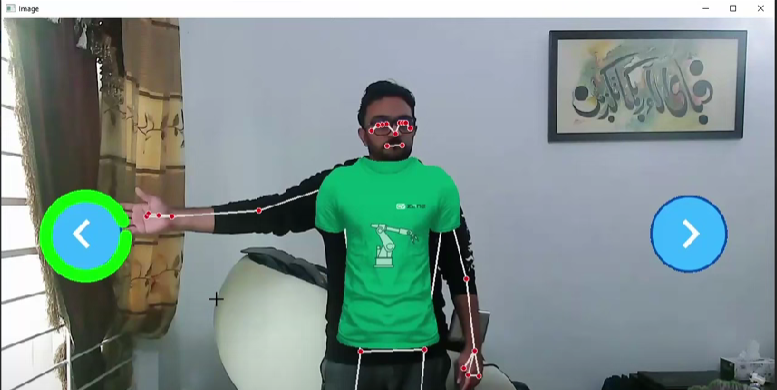
\includegraphics[angle=0, width=\textwidth]{gomlek2.PNG}
 	
 	\label{gomlek2}
 	Şekil \ref{gomlek2} de kişi sağ elini buton hizasında belli bir süre kaldırdığında butonun çevresinde yeşil bir daire oluşur.\cite{TisortPackage}	
 	
 	
 \end{figure}
 \newpage
 \begin{figure}[!ht]
 	\caption{}
 	\centering
 	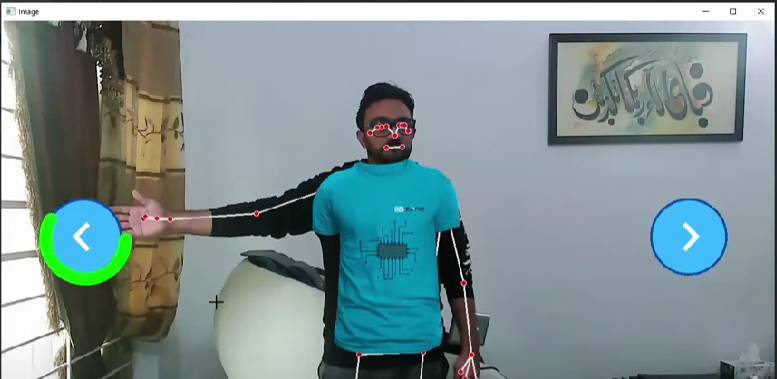
\includegraphics[angle=0, width=\textwidth]{gomlek3Sol.PNG}
 	
 	\label{gomlek3}
 	Şekil \ref{gomlek3} de kişi sağ elini buton hizasında kaldırdığında sonraki tişört gösterilmiştir\cite{TisortPackage}.	
 \end{figure}
 
 \begin{figure}[!ht]
 	\caption{}
 	\centering
 	\includegraphics[angle=0, width=\textwidth]{gomlek4Sol.PNG}
 	
 	\label{gomlek4}
 	Şekil \ref{gomlek4} de kişi sağ elini buton hizasında kaldırdığında sonraki tişört gösterilmiştir\cite{TisortPackage}.	
 \end{figure}
 \newpage
 \begin{figure}[!ht]
 	\caption{}
 	\centering
 	\includegraphics[angle=0, width=\textwidth]{gomlek1Sag.PNG}
 	
 	\label{gomlek5}
 	Şekil \ref{gomlek5}de kişi sol elini buton hizasında belli bir süre kaldırdığında butonun çevresinde yeşil bir daire oluşur.\cite{TisortPackage}	
 \end{figure}
 \begin{figure}[!ht]
 	\caption{}
 	\centering
 	\includegraphics[angle=0, width=\textwidth]{gomlek2Sag.PNG}
 	
 	\label{gomlek6}
 	Şekil \ref{gomlek6}  kişi sol elini buton hizasında kaldırdığında sonraki tişört gösterilmiştir\cite{TisortPackage}.	
 \end{figure}
 \begin{figure}[!ht]
 	\caption{}
 	\centering
 	\includegraphics[angle=0, width=\textwidth]{gomlekSagSol1.PNG}
 	
 	\label{gomlek7}
 	Şekil \ref{gomlek7}  kişi sağ elini buton hizasında belli bir süre kaldırdığında butonun çevresinde yeşil bir daire oluşur\cite{TisortPackage}.	
 \end{figure}
 \newpage
 \begin{figure}[!ht]
 	\caption{}
 	\centering
 	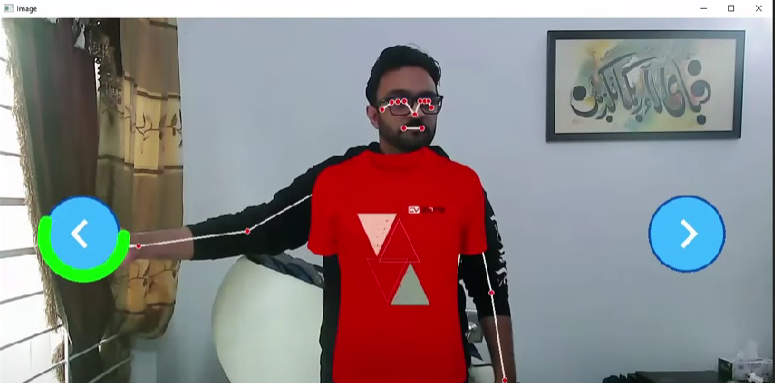
\includegraphics[angle=0, width=\textwidth]{gomlekSagSol2.PNG}
 	
 	\label{gomlek8}
 	Şekil \ref{gomlek8} de bir önceki tişört olan kırmızı renki tişört gösteriliyor\cite{TisortPackage}.	
 \end{figure}
 \newpage
 
 
 \title{Antropometrik Olçüme Göre
 	Mediapipe İskeletini Düzenleme
 	Raporu Hafta 7}
 \author{}
 \date{}
 \maketitle
 \setcounter{section}{0}
 \begin{abstract}
 	\begin{justify}
 		Bu çalışma, insan vücudunun antropometrik ölçümlerine göre Mediapipe iskeletinin düzenlenmesini ele almaktadır. Antropometri, insan vücudunun ölçüleri ile ilgilenen bir tekniktir. Çalışmanın amacı, Mediapipe iskelet modelinin antropometrik referans noktaları kullanılarak daha doğru ve gerçekçi bir şekilde düzenlenmesidir. Çalışmada, vücut hareketsiz ve belirli bir standart pozisyondayken alınan yapısal vücut ölçüleri kullanılmıştır. Mediapipe algoritması kullanılarak elde edilen sonuçlar, insan vücudunun çeşitli bölümleri için yapılan ölçümlerle karşılaştırılmıştır. Sonuçlar, düzenlenen iskelet modelinin daha yüksek doğruluk ve performans gösterdiğini ortaya koymuştur. Çalışmada yapılan karşılaştırmalar sonucunda, antropometrik ölçümlerin iskelet modellemeye olan katkıları vurgulanmıştır.
 	\end{justify}
 	\textbf{Anahtar Kelimeler:}  Antropometri, Mediapipe, iskelet düzenleme, yapısal vücut ölçüleri
 	
 	
 \end{abstract}
\section{Giriş}
Antropometri, insan vücudunun ölçüleri ile ilgilenen bir tekniktir ve bireyler veya gruplar arasında anatomi, coğrafi bölge ve meslek grupları gibi çeşitli faktörlerden kaynaklanan farklılıkları ve benzerlikleri saptayarak daha geniş bir insan kitlesine uygun tasarımlar yapma imkanı sağlar. Çalışmamızın motivasyonu, mevcut Mediapipe iskelet modelinin antropometrik referans noktaları kullanılarak daha doğru ve gerçekçi hale getirilmesidir. Önceki çalışmalarda, vücut ölçülerinin iskelet modellerine entegrasyonu yeterince ele alınmamış, bu da modellerin doğruluğunu sınırlamıştır \cite{Antropometrik}.

Bu çalışma, Mediapipe iskelet modelinin antropometrik ölçümlerle düzenlenmesine odaklanmıştır. Literatüre katkımız, insan vücudunun belirli referans noktaları kullanılarak iskelet modelinin daha yüksek doğrulukla düzenlenmesini sağlamaktır.
\section{VERİ/DENEYSEL ÇALIŞMA DÜZENEĞİ VEYA LİTERATÜR ARAŞTIRMASI}
Kullanılan veri, insan vücudunun belirli referans noktalarına dayanan antropometrik ölçümlerden oluşmaktadır. Deneysel çalışmada, bu ölçümler kullanılarak Mediapipe iskelet modeli düzenlenmiştir. Verilerin elde edilme amacı, iskelet modelinin doğruluğunu arttırmaktır\cite{Antropometrik}.
 \section{Referans Noktaları}

Antropometrik ölçümlerin standartlaştırılması amacıyla bazı referans noktaları belirlenmiştir:
\begin{enumerate}
	\item Yedinci boyun omuru (cervicale noktası)
	\item Ense kökü
	\item Yan boyun başlangıcı
	\item Omuz başı (acromion noktası)
	\item Omuz ortası
	\item Arka kol başlangıcı (triceps)
	\item Maksimum pazu kesiti
	\item Dirsek (olecranon)
	\item Bilek kesiti
	\item El başlangıcı
	\item Başparmak başlangıcı
	\item Kasların simetri merkezi
	\item Şakaklar
	\item Alt çene ucu(gnathion)
	\item Ön boyun üstü
	\item Ön boyun altı
	\item Bel çizgisi
	\item Kalça çizgisi
	\item Dizkapağı üstü
	\item Dizkapağı altı
	\item Ayak bileği kesiti(malleolus)
	\item Ayak tabanı
	\item Tepe noktası(vertex)
	\item Göğüs çizgisi\cite{Antropometrik}.
\end{enumerate}
\section{Yapısal Vücut Ölçüleri}
Yapısal vücut ölçüleri
Vücudun, ayakta ve oturarak belirli standart duruşlarında elde edilen değerlerdir.
\begin{enumerate}
	\item  Yükseklikler : Aytaktayken yerden, otururken oturma yüzeyinden ilgili vücut noktasına kadar olan uzunluklardır.  Dikey düzlemde ölçülürler.
	\item Genişlikler : Yatay ve enine çaplardır. Dikey düzlemde ölçülürler.
	\item Derinlikler : Yatay ve dikine çaplardır. Yanal düzlemde ölçülürler.
	\item Uzunluklar : Herhangi bir vücut kısmının uzun ekseni boyunca ölçülen değerdir.
	\item Çevresel uzunluklar : Bir vücut parçasının kendisiyle aynı düzlemdeki çevresidir.
\end{enumerate}
Eğrisel uzunluklar
\begin{enumerate}
	\item Düşüklükler : Boyun, göğüs, bel ve kalça arasındaki mesafelerdir.
\end{enumerate}
Kalınlıklar
\begin{enumerate}
	\item Çıkıntılar : Bir vücut bileşeninin ucunun bileşenin başlangıcına olan uzaklığıdır \cite{Antropometrik}.
\end{enumerate}
\newpage
  \begin{figure}[!ht]
	\caption{}
	\centering
	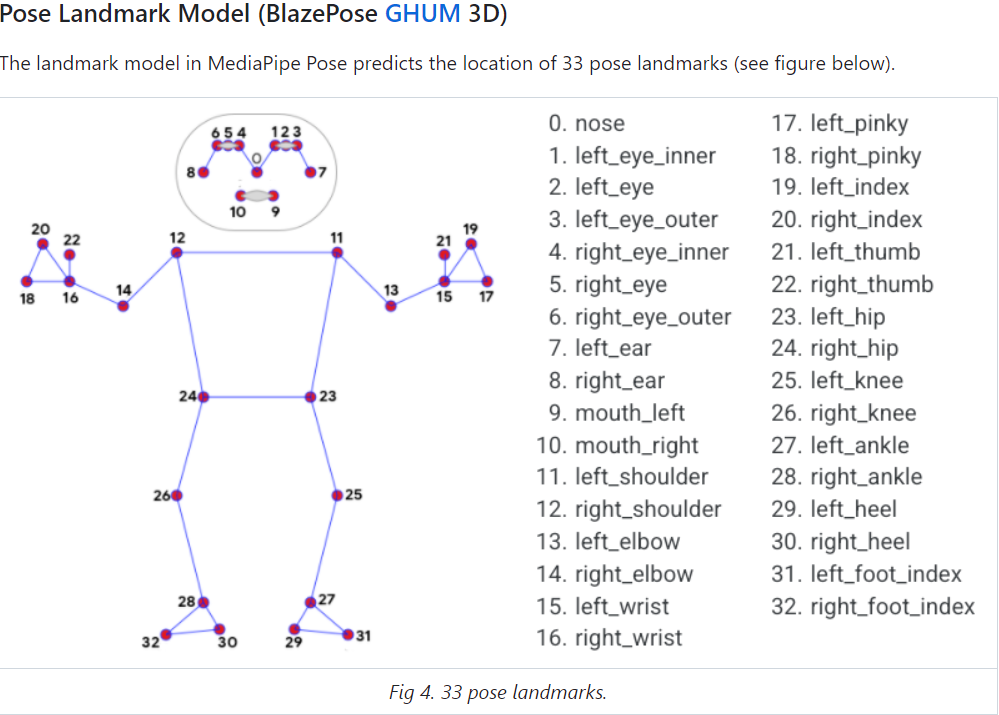
\includegraphics[width=0.8\textwidth]{mediapipe_iskelet.PNG}
	\label{CVZonex}
	Şekil \ref{CVZonex} de mediaPipe iskeleti gösterilmiştir\cite{MediapipeGithubb}.	
	
	
	
\end{figure}
\newpage
\begin{figure}[!ht]
	\caption{}
	\centering
	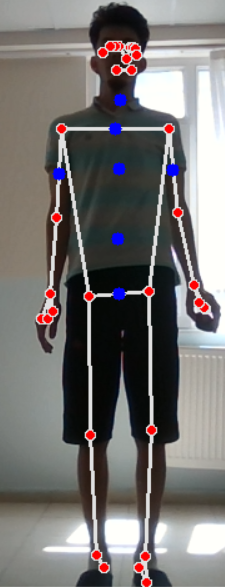
\includegraphics[width=0.4\textwidth]{mediapipeBen.PNG}
	\label{mediapipeBen}
	
	
	Şekil \ref{mediapipeBen} Antropometrik ölçümler kullanılarak mediaPipe iskeletinde yeni noktalar gösterilmiştir.	
	
	
	\newpage
\end{figure}

\section{Yöntem}
Çalışmada, Mediapipe algoritması kullanılarak antropometrik ölçümlerle iskelet modelinin düzenlenmesi gerçekleştirilmiştir. Veri, insan vücudunun belirli referans noktalarından alınan ölçümlerden oluşmaktadır. Bu ölçümler, iskelet modelinin daha doğru ve gerçekçi bir şekilde düzenlenmesi için kullanılmıştır. Kullanılan yöntemlerin başarımı, ölçüm metrikleri ile değerlendirilmiştir.
\newpage
\section{Orta Nokta }
Bir doğru parçasının üzerinde A ve B noktaları bulunuyor olsun. Bu noktalara eşit uzunlukta ve aynı doğrultuda olan bir C noktası alındığında bu noktaya orta nokta denir.

\begin{figure}[!ht]
	\caption{}
	\centering
	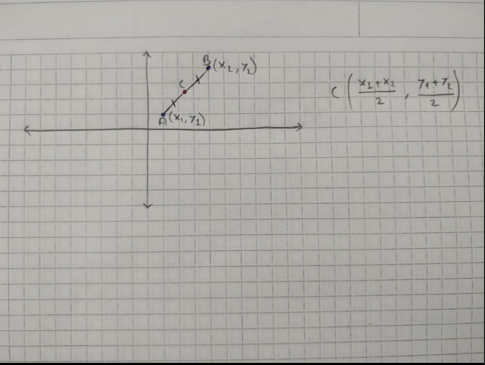
\includegraphics[width=0.5\textwidth]{ortaNokta.PNG}
	\label{OrtaNokta}
	
	
	Şekil \ref{OrtaNokta} Orta noktanın formülü gösterilmiştir.	
	
	
	
\end{figure}


\section{İki Nokta Arası Uzaklık }
Analitik düzlemde, verilen A(x1,y1) ve B(x2,y2) noktaları için ilk adımımız her iki noktadan da eksenlere dik çizmek olacaktır. Bu, her iki noktayı da eksenlerle kesiştirecektir. Ardından, bu kesişim noktalarını birleştirerek, A ve B noktalarını birleştiren bir doğru elde ederiz. Bu doğru, eksenlere dik çizdiğimiz doğrular ile birlikte bir dik üçgen oluşturur (ABC). Bu dik üçgenin dik kenar uzunlukları, eksenlerdeki kesişim noktalarının farkına eşit olacaktır. Daha sonra, bu dik kenarların uzunluklarını belirleyerek Pisagor teoremi uygulanarak hipotenüs uzunluğunu hesaplarız ve sonuç olarak iki nokta arasındaki uzaklığı buluruz.

\begin{figure}[!ht]
	\caption{}
	\centering
	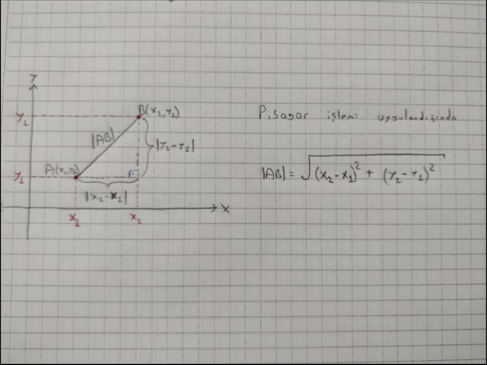
\includegraphics[width=0.5\textwidth]{ikiNoktaArasiUzaklik.PNG}
	\label{ikiNoktaArasiUzaklık}
	
	
	Şekil \ref{ikiNoktaArasiUzaklık} iki nokta arası uzaklığın formülü gösterilmiştir.	
	
	
	
\end{figure}
\newpage

\section{Sonuç}
Bu çalışma ile Mediapipe iskelet modeli, antropometrik ölçümler kullanılarak daha doğru ve gerçekçi bir şekilde düzenlenmiştir. Elde edilen sonuçlar, modelin doğruluğunu arttırmış ve diğer çalışmalardan farklı olarak antropometrik referans noktalarını kullanmanın önemini vurgulamıştır.
\title{Poz Tespiti ve Görsel Ögelerin Eklenmesi 
	Programı Raporu Hafta 8}
\author{}
\date{}
\maketitle
\setcounter{section}{0}
 \begin{abstract}
	\begin{justify}
	Bu rapor, Python dilinde yazılmış poz tespiti ve görsel öğelerin eklenmesi programını incelemektedir. Program, MediaPipe ve OpenCV kütüphanelerini kullanarak insan vücudunun belirli noktalarını tespit eder ve bu tespit sonuçlarını kullanarak görsel öğeleri canlı videoya ekler. Programın işleyişi, kullanılan kütüphaneler ve programın eksiklikleri ele alınmıştır. Sonuçlar, poz tespiti ve görsel öğelerin eklenmesinde elde edilen başarıları ve karşılaşılan sorunları özetlemektedir.
	\end{justify}
	\textbf{Anahtar Kelimeler:}  Poz tespiti, MediaPipe, OpenCV, Python, görsel öğeler
	\section{Giriş}
	Bu rapor, Python programı olarak yazılmış olan poz tespiti ve görsel öğelerin eklenmesi programını incelemektedir. Program, MediaPipe kütüphanesi kullanılarak insan vücudunun belirli noktalarını tespit eder ve bu noktaları kullanarak omuzlar, boyun ve eller gibi görsel öğeleri canlı videoya ekler. Çalışmamızın motivasyonu, poz tespiti ve artırılmış gerçeklik uygulamalarında kullanılan yöntemleri incelemek ve bu alandaki mevcut çözümleri daha etkin hale getirmektir \cite{MediapipeGithubb}.
	\section{Kullanılan Kütüphaneler}
	Programın işlevselliğini sağlamak için aşağıdaki kütüphaneler kullanılmıştır:
	\begin{enumerate}
     \item 	OpenCV (cv2): Görüntü işleme ve kamera yakalama için kullanılır.
	 \item MediaPipe (mediapipe): Poz tespiti yapmak için kullanılır.
		
	\end{enumerate}
	\section{Program Akışı}
	Programın ana akışı aşağıdaki adımlardan oluşmaktadır:
	\begin{enumerate}

\item Gerekli kütüphanelerin yüklenmesi.
\item Poz tespiti modelinin yüklenmesi.
\item Kamera yakalayıcısının başlatılması.
\item Görsel öğelerin yüklenmesi ve boyutlarının ayarlanması.
\item Sonsuz bir döngüde:
     	\begin{enumerate}
     	\item	Kameradan bir kare alınması.
     	\item 	Gri tonlamalı görüntünün oluşturulması.
     	\item 	MediaPipe ile poz tespiti yapılması.
     	\item 	Elde edilen sonuçların işlenmesi.
     	\item 	Oluşturulan son görüntünün gösterilmesi.
     	\item 	Çıkış için ‘q’ tuşuna basılmasının beklenmesi.
     	\end{enumerate}
\end{enumerate}
\section{Programın İşlevselliği}
Program, MediaPipe kullanarak pozisyon tespiti yapar ve bu tespit sonuçlarını kullanarak görsel öğeleri canlı videoya ekler. İnsan vücudunun belirli noktalarını tespit eder ve bu noktaları kullanarak omuzlar, boyun ve eller gibi görsel öğeleri ekleyerek eğlenceli bir etki sağlar.

\section{Sonuç}
Bu rapor, Python dilinde yazılmış olan poz tespiti ve görsel öğelerin eklenmesi programını inceledi. Program, MediaPipe ve OpenCV gibi kütüphaneleri kullanarak insan vücudunun belirli noktalarını tespit eder ve bu tespit sonuçlarını kullanarak görsel öğeler ekler. Program, insan vücudunun belirli noktalarını doğru bir şekilde tespit etmede ve görsel öğeleri canlı videoya entegre etmede başarılıdır \cite{ChatGPT3.5}.	
	
\end{abstract}
\section{Programın Eksiklikleri}
	\begin{enumerate}
	\item Programda, MediaPipe iskeletinde resim eklenen belirli bir kısım görünmediğinde hata döndürüp programı sonlandırmaktadır.
	\item Bütün bir resim parçalara ayrıldığı için MediaPipe iskeletinde resimler birbirlerini tamamlamamaktadır.
	\item MediaPipe iskeletinin üzerinde oluşturulan dörtgen şeklindeki yerleştirilen resimde verilen alana resmi tam oturtma işlemi yapıldığından resim bulanık gözükmektedir.
\end{enumerate}
\newpage
\title{Program Eksikleri Giderme Hafta 9}
\author{}
\date{}
\maketitle
\setcounter{section}{0}
\begin{abstract}
	\begin{justify}
		Bu rapor, Python programı olarak yazılmış olan poz tespiti ve görsel öğelerin eklenmesi programının eksiklerine bulunan çözümleri incelemektedir. Program, MediaPipe kütüphanesi kullanılarak insan vücudunun belirli noktalarını tespit eder\cite{MediapipeGithubb}.
	\end{justify}
	\textbf{Anahtar Kelimeler:}  Antropometri, Mediapipe, iskelet düzenleme, yapısal vücut ölçüleri
	
	
\end{abstract}
	\section{Kullanılan Kütüphaneler}

Program, işlevselliği sağlamak için aşağıdaki kütüphaneleri kullanmaktadır:

\begin{itemize}
	\item OpenCV (\texttt{cv2}): Görüntü işleme ve kamera yakalama için kullanılır.
	\item MediaPipe (\texttt{mediapipe}): Poz tespiti yapmak için kullanılır.
\end{itemize}

\section{Program Akışı}

Programın ana akışı aşağıdaki adımlardan oluşur:

\begin{enumerate}
	\item Gerekli kütüphanelerin yüklenmesi.
	\item Poz tespiti modelinin yüklenmesi.
	\item Kamera yakalayıcısının başlatılması.
	\item Görsel öğelerin yüklenmesi ve boyutlarının ayarlanması.
	\item Sonsuz bir döngüde:
	\begin{itemize}
		\item Kameradan bir kare alınması.
		\item Gri tonlamalı görüntünün oluşturulması.
		\item Mediapipe ile pose tespiti yapılması.
		\item Elde edilen sonuçların işlenmesi.
		\item Oluşturulan son görüntünün gösterilmesi.
		\item Çıkış için 'q' tuşuna basılmasının beklenmesi.
	\end{itemize}
\end{enumerate}

\section{Programın İşlevselliği}

Program, MediaPipe kullanarak pozisyon tespiti yapar ve bu tespit sonuçlarını kullanarak görsel öğeleri canlı videoya ekler. İnsan vücudunun belirli noktalarını tespit eder ve bu noktaları kullanarak omuzlar, boyun ve eller gibi görsel öğeleri ekleyerek eğlenceli bir etki sağlar.

\section{Sonuç}

Bu rapor, Python dilinde yazılmış olan poze tespiti ve görsel öğelerin eklenmesi programını inceledi. Program, MediaPipe ve OpenCV gibi kütüphaneleri kullanarak insan vücudunun belirli noktalarını tespit eder ve bu tespit sonuçlarını kullanarak görsel ekler.\cite{ChatGPT3.5}.
\section{Programın Eksikleri}
\begin{enumerate}
	\item Bu programda kod çalıştığında mediapipe iskeletinde resim eklenen belirli bir kısım görünmediğinde hata döndürüp programı sonlandırır.
	\item Bütün bir resim parçala ayrıldığı için mediapipe iskeletinde resimlerin birbirlerini tamamlamıyor.
	\item Mediapipe iskeletinin üzerinde oluşturulan dörtgen şeklindeki yerleştirilen resimde verilen alana resimi tam oturtma işlemi yapıldığından resim bulanık gözüküyor.
	\item Mediapipe iskeletinin üzerine eklenen tişört kısımlarının arka planları gözüküyor.
	\newpage 
	
	
\end{enumerate}
\section{Çözümler}
\begin{enumerate}
	\item Bu programda kod çalıştığında mediapipe iskeletinde resim eklenen belirli bir kısım görünmediğinde hata döndürüp programı sonlandırır.
	
	\begin{figure}[!ht]
		\caption{}
		\centering
		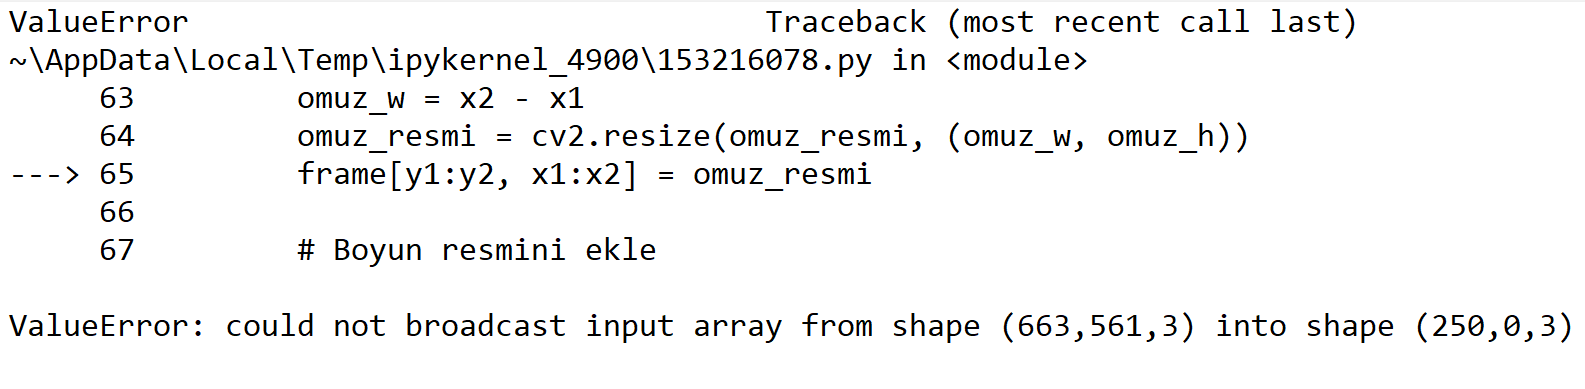
\includegraphics[width=0.7\textwidth]{Hata1mediapipe.PNG}
		\label{mediapipeHata1}
		
		
		Şekil \ref{mediapipeHata1} mediapipe iskeletinde belirli bir bölge algınmamasından dolayı alınan hatanın resmi gösterilmiştir.	
		
		
		
	\end{figure}
	\begin{figure}[!ht]
		\caption{}
		\centering
		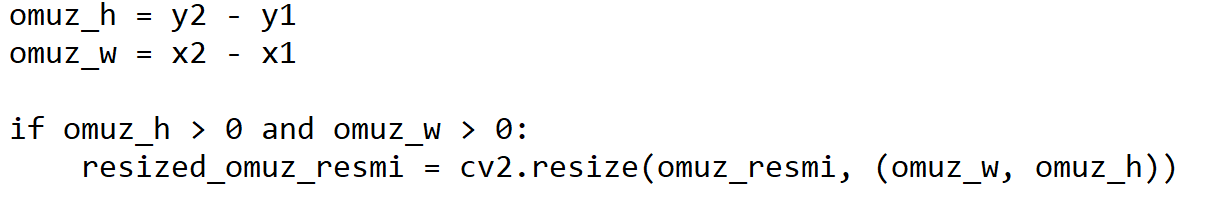
\includegraphics[width=0.7\textwidth]{cozumMediapipe1.PNG}
		\label{mediapipeCozum1}
		
		
		Şekil \ref{mediapipeCozum1} mediapipe iskeletinde omuz resminin yeniden boyutlandırma ve yerleştirme kodunun  resmi gösterilmiştir.	
		
		
		
	\end{figure}
	\begin{figure}[!ht]
		\caption{}
		\centering
		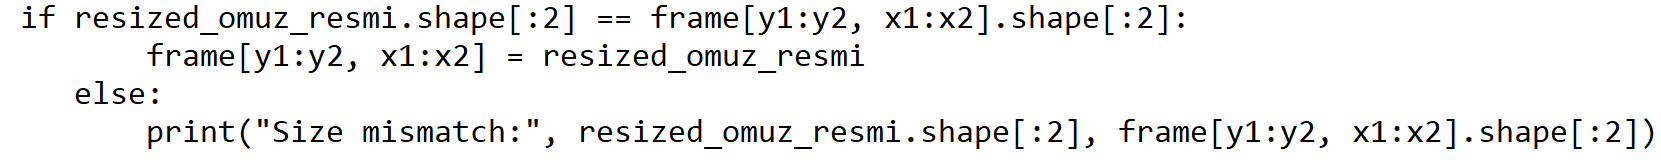
\includegraphics[width=0.7\textwidth]{mediapipeCozum2.PNG}
		\label{mediapipeCozum2}
		
		
		Şekil \ref{mediapipeCozum2} mediapipe iskeletindeki eklemler üzerine tişört parçaları  yerleştirmeden önce boyut kontrolü yapan kod gösterilmiştir.	
		
		
		
	\end{figure}
	\newpage
	\item Mediapipe iskeletinin üzerinde oluşturulan dörtgen şeklindeki yerleştirilen resimde verilen alana resimi tam oturtma işlemi yapıldığından resim bulanık gözüküyor.
	\begin{figure}[!ht]
		\caption{}
		\centering
		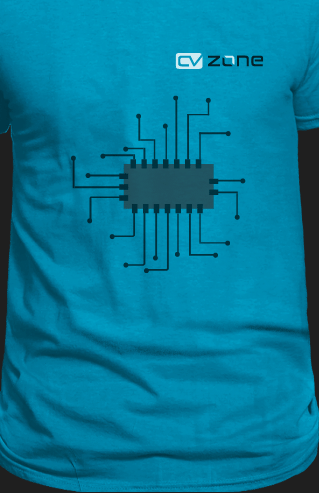
\includegraphics[height=0.7\textheight]{dikdortgen.PNG}
		\label{dikdortgen}
		
		
		Şekil \ref{dikdortgen} Mediapipe iskeletinde bulanık görünen tişörtün kısmı gösteriliyor\cite{MediapipeGithubb}.	
		
		
		
	\end{figure}
	\item Mediapipe iskeletinin üzerine eklenen tişört kısımlarının arka planları alfa kanalı eklenerek kaldırıldı\cite{ChatGPT3.5}.
	
\end{enumerate}
\begin{figure}[!ht]
	\caption{}
	\centering
	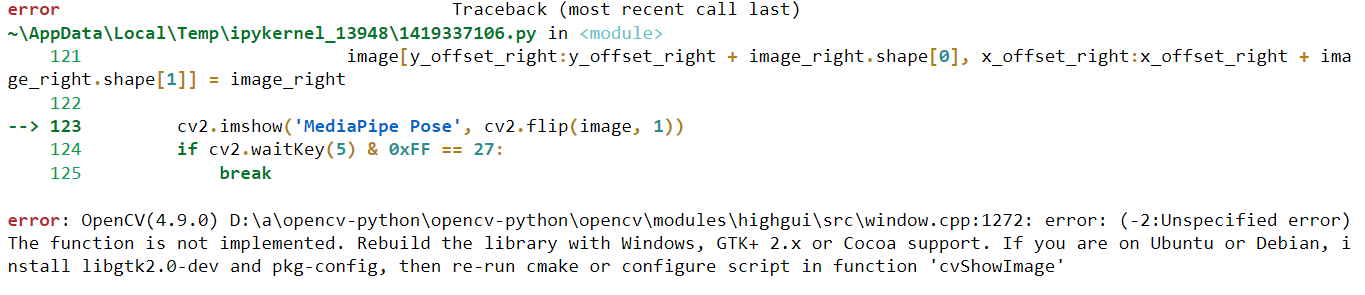
\includegraphics[width=0.7\textwidth]{MediapipeHata3.PNG}
	\label{mediapipeHata2}
	
	
	Şekil \ref{mediapipeHata2} Alınan hata gösterilmiştir.	
	
	
	
\end{figure}
\newpage
\begin{figure}[!ht]
	\caption{}
	\centering
	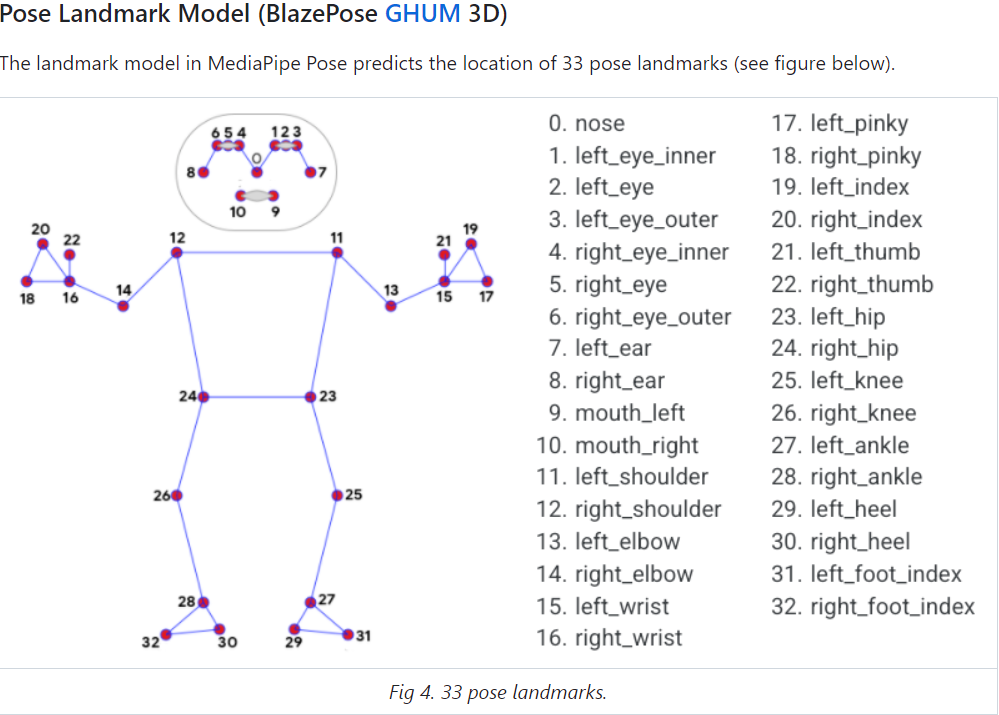
\includegraphics[width=0.7 \textwidth]{mediapipe_iskelet.PNG}
	\label{iskelet}
	
	
	Şekil \ref{iskelet} mediaPipe iskeleti gösterilmiştir\cite{MediapipeGithubb}.	
	
	
	
\end{figure}
\title{Poz Tespiti ve Görsel Öğelerin Eklenmesi 
	Programı Raporu Hafta 10}
\author{}
\date{}
\maketitle
\setcounter{section}{0}
\begin{abstract}
	\begin{justify}
	Bu rapor, Python dilinde geliştirilen ve Mediapipe ile OpenCV kütüphanelerini kullanarak poz tespiti ve görsel öğelerin eklenmesini gerçekleştiren bir uygulamanın tasarımını, kullanılan yöntemleri ve elde edilen sonuçları incelemektedir. Uygulama, Tkinter ile kullanıcı arayüzü sunmakta ve kullanıcıların seçtiği görüntüleri işleyerek, poz tespitine dayalı olarak gerçek zamanlı görüntü yerleştirme işlemlerini gerçekleştirmektedir.
	\end{justify}
	\textbf{Anahtar Kelimeler:} Poz tespiti, MediaPipe, OpenCV, Tkinter, görüntü işleme
	
	
\end{abstract}
\section{Giriş}
Bu rapor, görüntü işleme uygulamasının tasarımını, uygulanan yöntemleri ve elde edilen sonuçları açıklamaktadır. Uygulama, MediaPipe kütüphanesi ve OpenCV kullanılarak geliştirilmiş olup, bir kullanıcı arayüzü üzerinden görsel seçimini ve poz tespitini gerçekleştirir. Bu uygulamanın amacı, kullanıcıların seçtiği görüntüleri insan vücudunun belirli noktalarına yerleştirerek, eğlenceli ve etkileşimli bir deneyim sunmaktır.
\section{Gelişme}
İlk olarak, kullanıcıya üç farklı görüntü seti arasından seçim yapma olanağı sunmak için Tkinter kullanılarak bir arayüz oluşturulmuştur. Kullanıcı seçim yaptıktan sonra, seçilen görüntüler arka planı şeffaf hale getirme ve kırışıklıkları tespit etme işlemlerinden geçirilmiştir\cite{ChatGPT3.5}.
	\begin{enumerate}
\item Arka Planın Şeffaf Hale Getirilmesi: Renk aralığı belirlenerek OpenCV kullanılmış ve edge detection yöntemi ile kırışıklıklar tespit edilmiştir. Alpha maskesi ile kırışıklık maskesi birleştirilerek, görüntülerin arka planına uygun bir şekilde alpha kanalı eklenmiştir.

\item Poz Tespiti ve Görüntü Yerleştirme: MediaPipe kullanılarak poz tespiti yapılmış ve belirlenen pozlara göre görüntülerin belirli noktalara (omuz, boyun, sağ omuz ve sol omuz) yerleştirilmesi sağlanmıştır. İşlenen görüntüler, kamera görüntüsü üzerine bindirilerek, kullanıcıya gerçek zamanlı olarak gösterilmiştir.
\end{enumerate}
	\begin{figure}[!ht]
	\caption{}
	\centering
	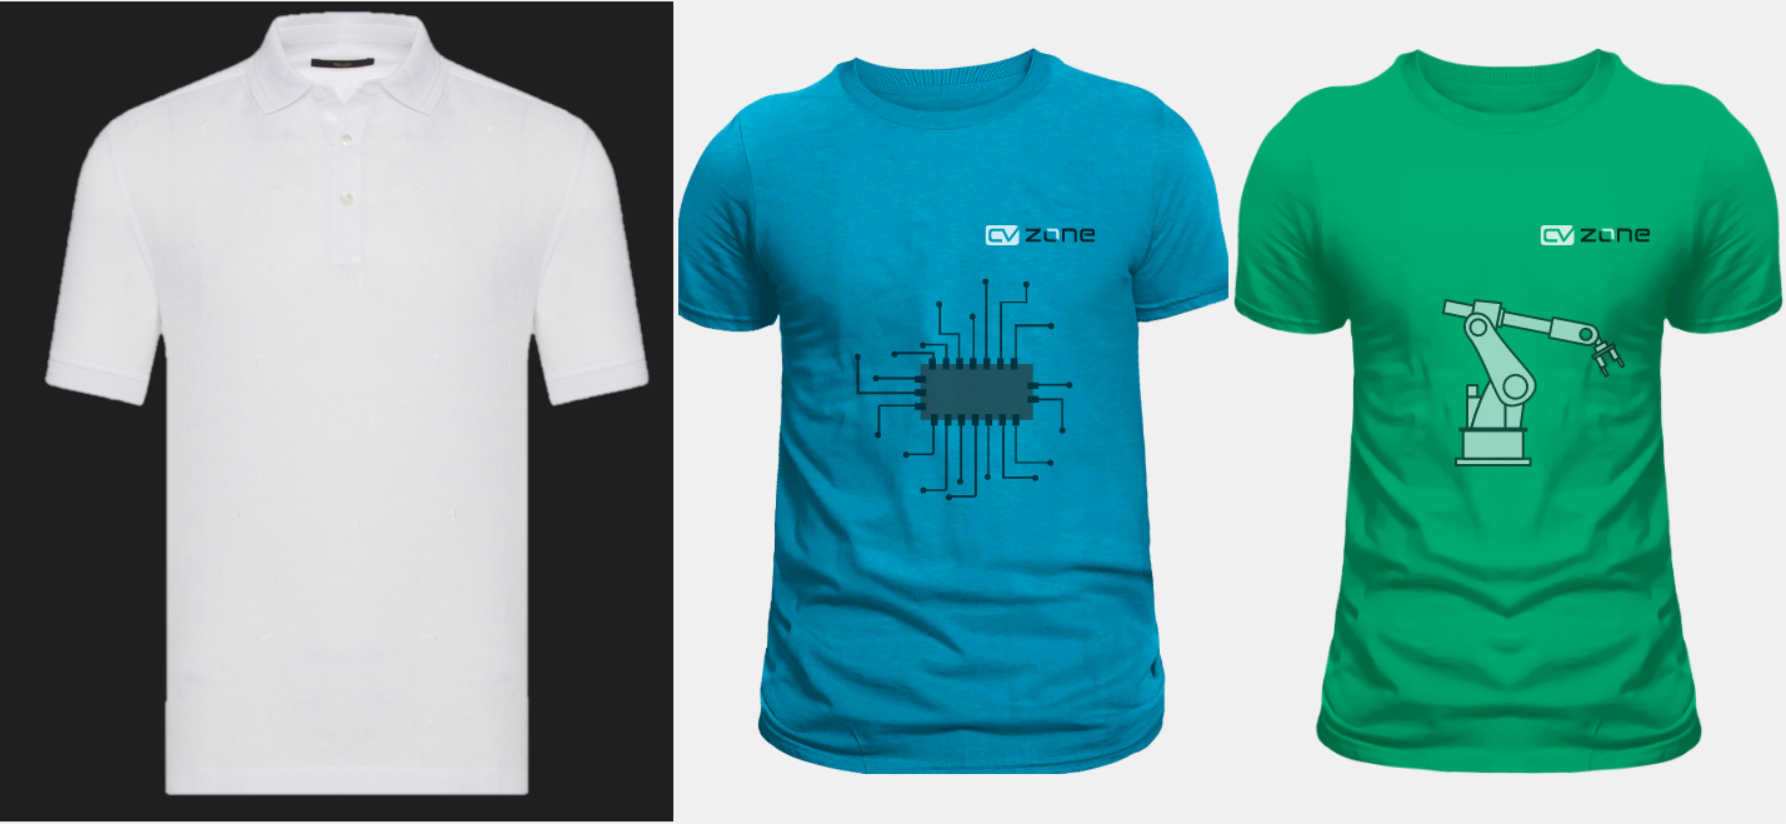
\includegraphics[width=0.7\textwidth]{Tkinter.PNG}
	\label{tikinter}
	
	
	Şekil \ref{tikinter} tikinter kullanılarak oluşturulmuş arayüz gösterilmiştir\cite{MediapipeGithubb}.	
	
	
	
\end{figure}
\begin{figure}[!ht]
	\caption{}
	\centering
	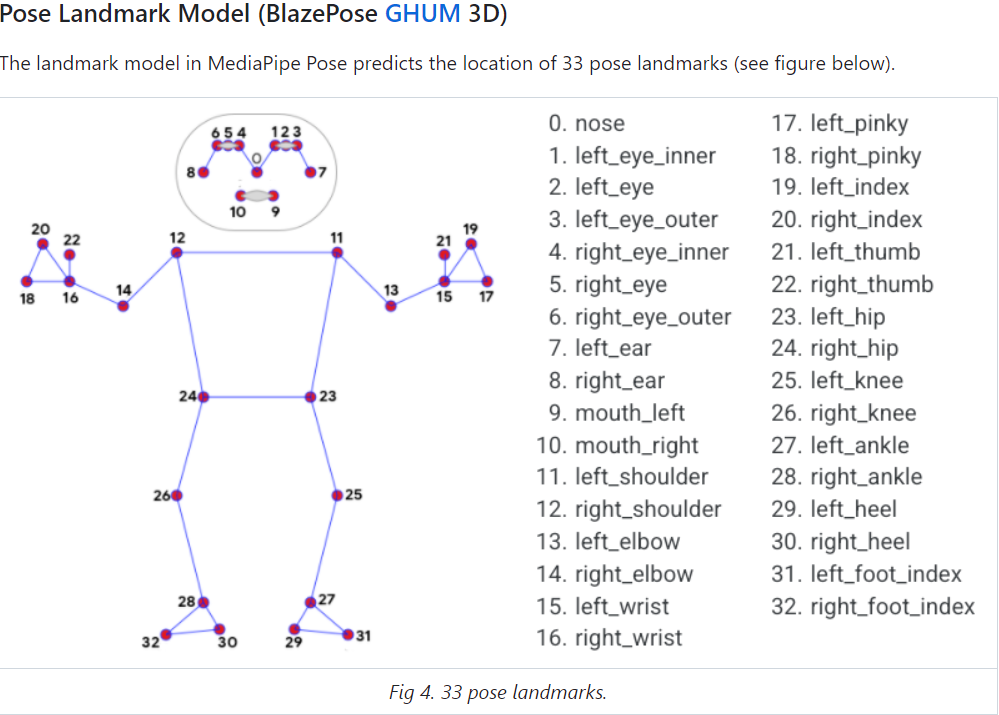
\includegraphics[width=0.7\textwidth]{mediapipe_iskelet.PNG}
	\label{iskeletm}
	
	
	Şekil \ref{iskeletm} mediaPipe iskeleti gösterilmiştir\cite{MediapipeGithubb}.	
	
	
	
\end{figure}
\newpage

\section{Sonuç}
Geliştirilen görüntü işleme uygulaması, kullanıcı dostu bir arayüz üzerinden kolayca kullanılabilir ve gerçek zamanlı olarak poz tespiti ve görüntü yerleştirme işlemlerini gerçekleştirir. Kullanıcılar, seçtikleri görüntü setlerini kullanarak farklı deneyimler elde edebilirler. Uygulamanın genel performansı ve görüntü işleme sonuçları, beklentileri karşılayacak düzeydedir.
\newpage
	%Kaynakçayı yazdırmak
	\bibliographystyle{ieeetr}
	\bibliography{references.bib} 
	%\printbibliography %Prints bibliography
	
	
	
\end{document}